
% Para el análisis y ajuste se trabajó con dos conjuntos de datos distintos. El primero fue el conjunto de datos que la colaboración Pierre Auger presentó en la Conferencia Internacional de Rayos Cósmicos (ICRC) del año 2015, este conjunto de datos se utilizó para el cálculo de las correcciones climáticas al estimador de energía \cite{aab2017impact}. El segundo conjunto de datos se presentó en la ICRC del año 2019. Entre estos dos conjuntos de datos existieron cambios en la reconstrucción de energía de los eventos, en particular en el valor de la señal de S$(1000)$ \cite{isabel}, además de agregar la corrección por las modulaciones del clima propuesto en \cite{aab2017impact} sobre este mismo valor de señal y se implementó una función de corte de intensidad constante CIC que varía en función de la energía. El objetivo de este capítulo es comprobar si la corrección del clima de la reconstrucción de eventos es adecuada.

\section{La física detrás de la modulación del clima}\label{seccion:fisica_clima}

El arreglo principal mide las 24 horas del día las lluvias de partículas que llegan al suelo. Las señales registradas por los WCDs, ya sea mediante la componente electromagnética o muónica de las EAS, se usan para determinan la posición del núcleo, la dirección de arribo del CR y la energía del primario. La señal de los eventos son ajustados mediante un función de distribución lateral (LDF) para obtener una señal de referencia $S(1000)$. Existieron cambios en los parámetros de la LDF y, por lo tanto, de valor de $S_{38}$, utilizado para estimar la energía del primario. La conversión de $S(1000)$ a $S_{38}$ se realiza mediante el método de corte de intensidad constante (CIC) explicado anteriormente. Además en la nueva reconstrucción el CIC es función de la energía.

\subsection{Trabajos anteriores}

Debido a la modulación del clima dependiente de la estaciones, es de esperarse encontrar una modulación diaria y anual sobre la cantidad de eventos observados por el SD. Ya que en días con menor densidad y presión atmosférica, los tanques detectan eventos por debajo del umbral con mayor facilidad. Este fenómeno fue estudiado por trabajos anteriores realizados por la colaboración Pierre Auger \cite{aab2017impact} \cite{collaboration2009atmospheric}. En particular, el trabajo \cite{aab2017impact} consideró el retraso que tienen los cambios de  la temperatura a distintas alturas sobre la superficie, como se muestra en la Fig\,\ref{fig:delay} que son datos del GDAS (Global Data Assimilation System) promediados por hora del día. Posteriormente esta corrección fue implementada en el proceso  de análisis de datos del observatorio.


En la Fig.\,\ref{fig:delay} se observa que los ajustes realizados a las variaciones de la temperatura  según la hora del día con una función del tipo $T(t) = T_{media} + A\times \sin((t-t_d)\nicefrac{\pi}{12\,\text{hs}})$.  En la Tabla\,\ref{tabla:delay} se observa que entre 1400\,m (altitud del observatorio Pierre Auger) y la mayor altitud medida por el GDAS existe un corrimiento de $2.1\pm0.7\,$hs.

Como la relación entre la densidad y la temperatura del aire están relacionadas mediante la expresión $\rho \approx \nicefrac{0.3484P}{T +273.16}\,$kgm$^{-3}$, con P en hPa y T en  $^o$C \cite{aab2017impact}, el corrimiento de la temperatura al aumentar la altitud también se ve reflejada en la densidad. Como la misma es una variable importante para el desarrollo de la cascada en al atmósfera, este retraso debe tenerse en cuenta.

\begin{figure}[H]
	\centering
	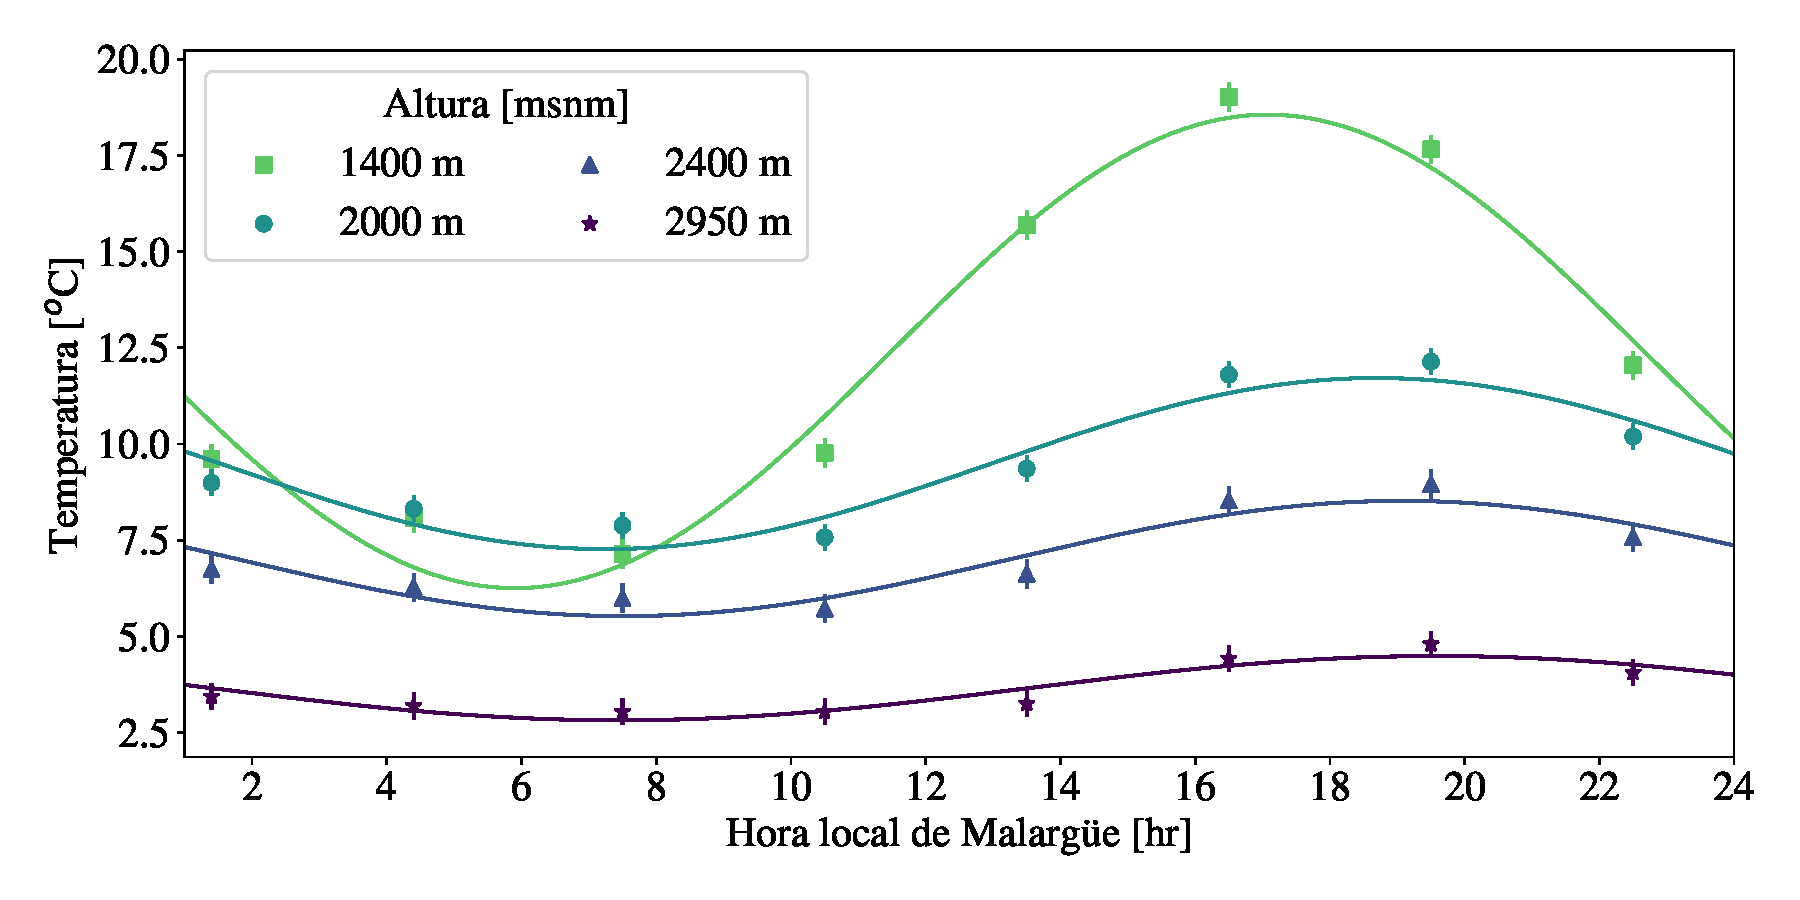
\includegraphics[width=0.8\textwidth]{delay_v2.pdf}
	\caption{Mediciones de la temperatura a distintas alturas sobre el nivel del mar en función de la hora del día en Malargüe. (Hora Local: GMT-3).}
	\label{fig:delay}
\end{figure}
\begin{table}[H]
\centering
\begin{tabular}{|c|c|c|c|}
	\hline
	\multirow{2}{*}{\begin{tabular}[c]{@{}c@{}}Altura \\ {[}msnm{]}\end{tabular}} & \multirow{2}{*}{\begin{tabular}[c]{@{}c@{}}T$_{media}$ \\ {[}$^o$C{]}\end{tabular}} & \multirow{2}{*}{A {[}$^o$C{]}} & \multirow{2}{*}{t$_d$ {[}h{]}} \\
																				  &                                                                                                      &                                                 &                                \\ \hline
	1400                                                                          & $12.4\pm0.5$                                                                                         & $5.6\pm0.6$                                     & $12.5\pm0.5$                   \\ \hline
	2000                                                                          & $9.5\pm0.2$                                                                                          & $2.1\pm0.3$                                     & $10.8\pm0.6$                   \\ \hline
	2400                                                                          & $7.0\pm0.2$                                                                                          & $1.4\pm0.2$                                     & $10.7\pm0.6$                   \\ \hline
	2950                                                                          & $3.7\pm0.1$                                                                                          & $0.8\pm0.1$                                     & $10.4\pm0.6$                   \\ \hline
	\end{tabular}
\caption{Características de la modulación de la temperatura en función de la altura sobre el nivel del mar.}\label{tabla:delay}
\end{table}

\subsection{Efectos de la atmósfera sobre los rayos cósmicos}

La variación de las condiciones atmosféricas afecta las señales de las lluvias atmosféricas extendidas. Estas señales pueden ser detectadas en la superficie por un arreglo de detectores, como los que se encuentran en el Observatorio Pierre Auger. Estos efectos pueden inducir errores sistemáticos en la reconstrucción de energía de los rayos cósmicos. Se han realizado  trabajos anteriores sobre los efectos del clima sobre la señal detectada en el Observatorio Pierre Auger \cite{collaboration2009atmospheric} \cite{aab2017impact}. En este trabajo se estudió eventos con energía mayor a $1\,$EeV entre los años 2005-2018, extendiendo los periodos de tiempo estudiados anteriormente.
%444444444444444444444444444

Para entender los parámetros utilizados para describir a la lluvia, debemos entender que son la longitud de radiación $X_0$, la profundidad de la lluvia $X_{max}$ y el radio de Molière $r_M$. La longitud de radiación definida como $X_0=\nicefrac{d}{2}$,  donde $d$ es un parámetro que indica cuanta cantidad de materia debe atravesar un partícula cargada relativista para perder un factor de $\approx 50\%$ de su  energía. El $X_0$ depende del material que atraviesa la partícula, y tiene unidades de [g\,cm$^{-2}$]. La profundidad de la lluvia $X_{max}$ de una cascada puramente electromagnética, i.e. iniciada por un fotón, tiene la siguiente expresión \cite{matthews2005heitler}
\begin{equation}
 	X_{max} = X_0{ln(\frac{E}{\xi^e_c})}
 \end{equation} 
donde  $\xi^e_c$ es la energía crítica para la cual las pérdida de energía por radiación supera a la pérdidad de energía por colisión, en el aire $\xi^e_c=85\,$MeV. Por último, el radio de Molière $r_M$ que puede expresarse como 
\begin{equation}
	r_M= \frac{E_s}{\xi^e_c}\frac{X_0}{\rho}
\end{equation}
es la máxima profundidad transversal que alcanza la lluvia. El valor de $E_s\approx21\,$MeV caracteriza las pérdidas por dispersión. Usualmente un cilindro con un radio $r_M$ contiene al 90\% de la energía depositada en la atmósfera por el primario. El radio de Molière local en el aire para una altura $h$ puede definirse como $r_M = \nicefrac{9.6\,\text{gcm}^{-2}}{\rho(h)}$ \cite{gora2006universal}. 
%444444444444444444444444444

Las variables atmosféricas importantes que afectan al desarrollo de la EAS en la atmósfera son la presión y la densidad del aire. Por un lado la presión es una medida de cantidad de materia que atraviesa el CR. Si la presión sobre la superficie aumenta implica que la lluvia va a atravesar más partículas, y por el contrario si la presión disminuye la lluvia tiene menos materia para interactuar. Esto afecta el desarrollo longitudinal de la lluvia cuando llega a la superficie. En la Fig.\,\ref{fig:eas} se muestran una esquema simplificado de las interacciones en al atmósfera de un primario de la misma energía. En la figura de la izquierda representa la lluvia donde la presión y la densidad está por encima de la media, y la figura de la derecha representa un lluvia donde la presión y la densidad de la atmósfera están por debajo de la media.

\begin{figure}[H]
	\centering
	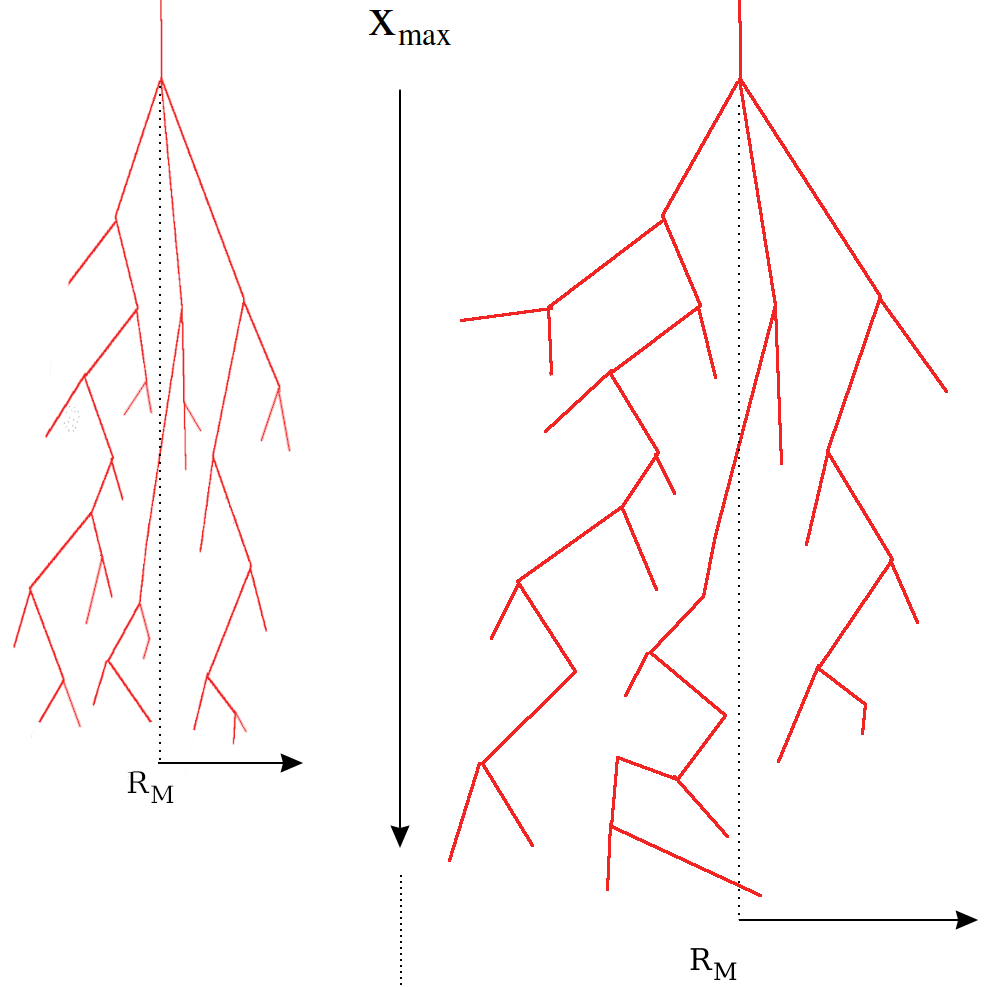
\includegraphics[width=0.5\textwidth]{eas.png}
	\caption{Diagramas simplificado de un lluvia de la misma energía para distintas condiciones atmosféricas}
	\label{fig:eas}
\end{figure}

Estos efectos se ven reflejados en la señal sobre el SD del Observatorio Pierre Auger. La extensión de la señal sobre el SD, es decir el $r_M$ puede cambiar según la densidad de la atmósfera por encima del SD. Los valores de $r_M$ relevantes para la señal medida son a nivel del suelo y a 1000 m. Esto implica que las variaciones de densidad (o de temperatura) a estas alturas están relacionadas con las variaciones al nivel del suelo. La variación a $\sim2400\,$m sobre el nivel del mar está atrasada dos horas con respecto a la variación sobre el Observatorio, que se encuentra a $\sim1400\,$m sobre el nivel del mar. Otro aspecto importante es que la amplitud de está variación disminuye con la altura. Entre las dos altitudes mencionadas existen una relación de aproximadamente $\nicefrac{1}{3}$ entre las amplitudes. 

\subsection{Descripción del modulación en la señal medida}

Considerando lo analizado en \cite{aab2017impact} \cite{collaboration2009atmospheric}, en este trabajo se propone la siguiente modulación, presentada en la Ec.\,\ref{eq:signal}, para la señal S que reciben los tanques 
\begin{equation}
	S=S_0\big(1+\alpha_P(P-P_0) +\alpha_{\rho}(\rho_{media}-\rho_0) + \beta_{\rho}(\rho_{2h}-\rho_{media})\big)
	\label{eq:signal}
\end{equation}
donde $S_0$ es la señal  del evento en condiciones atmosféricas medias, $P$ es la presión en el momento del evento, $P_0=862\,$hPa es la presión media en el rango de tiempo estudiado, $\rho_{media}$ es la densidad  media del aire en 24\,hs, $\rho_0=1.06\,$kgm$^{-3}$ es la densidad media durante el periodo estudiado, $\rho_{2h}$ es la densidad que se midió dos horas antes del evento  y los coeficientes $\alpha$ y $\beta$ tiene en cuenta la modulación del clima sobre la señal.  Si consideramos la tasa $R_{ang}$  por ángulo sólido $\Omega$

\begin{equation}
	\frac{dR_{ang}}{d\Omega} = \int_{S_{min}}^{\infty} P_{Tr}(S,\theta) d\Phi_{CR}
	\label{eq:rate_angular}
\end{equation}
donde $P_{Tr}$ es la probabilidad de que sea detectado un evento para un valor de señal mínimo $S_{min}$ dado, y $\Phi_{CR}$ es la densidad de eventos por ángulo sólido. La función $P_{Tr}$ tiene en cuenta la eficiencia del disparo de los tanques en función de la energía. Por ejemplo, para el SD 1500 m, como se mencionó anteriormente, la eficiencia máxima de disparo es a partir  de $3\,$EeV. Considerando  las Ecs.\,\ref{eq:s38_energy} y \ref{eq:expresion1} , se puede reescribir la Ec.\ref{eq:rate_angular} como integral de la señal medida S. Teniendo en cuenta que la corrección del clima es pequeña podemos escribir la Ec.\,\ref{eq:signal} como $S=S_0(1+\epsilon)$ y las Ecs. \ref{eq:expresion1} y \ref{eq:s38_energy}.
\begin{align*}
\frac{d\Phi_{CR}}{dE} 	&\propto E^{-\gamma} 					\qquad\qquad\qquad\qquad\qquad \quad \qquad \qquad		\frac{dE}{dS}  			= \frac{dE}{dS_0}\,\frac{dS_0}{dS}\\ 
					  	&= S^{-B\gamma}(1+\epsilon)^{B\gamma}    \qquad\qquad \qquad\qquad\qquad \qquad 				  	 = AB\,S^{B-1}\, (1+\epsilon)^{-B}\\
   		    			\frac{dR_{ang}}{d\Omega} &= \int_{S_{min}}^{\infty} P_{Tr}(S,\theta) \frac{d\Phi_{CR}}{dE} \frac{dE}{dS} dS\\
    						 &\propto \int_{S_{min}}^{\infty} P_{Tr}(S,\theta) \bigg( S^{-B\gamma}(1+\epsilon)^{B\gamma}\bigg) \bigg( AB\,S^{B-1}\, (1+\epsilon)^{-B}\bigg)dS\\
    						 &\propto A\,B (1+\epsilon)^{B\gamma - B}\int_{S_{min}}^{\infty} P_{Tr}(S,\theta) S^{-B\gamma +B -1} dS\\
\end{align*}

Dado que $\epsilon\,\ll\,1$, uno puede expandir la expresión $(1+\epsilon)^{B\gamma}$ hasta primer orden 
\begin{equation*}
	(1+\epsilon)^{B\gamma-B} \approx 1 + B(\gamma-1)\epsilon
\end{equation*}

Por lo que la expresión final queda de la siguiente forma

\begin{equation*}
	\frac{dR_{ang}}{d\Omega} \propto AB(1+B(\gamma - 1)\epsilon)\int_{S_{min}}^{\infty} P_{Tr}(S,\theta) S^{-B\gamma +B -1} dS
\end{equation*}

Considerando que $d\Omega= sin(\theta)d\theta d\phi$ y que el área efectiva  que tiene el observatorio para dado un evento con ángulo cenital $\theta$ es $M_{eff}=M\times cos(\theta)$, donde $M$ es el área activa del observatorio en el momento del evento. Podemos redefinir la tasa por área $R$ como

\begin{align*}
	dR 	&\propto \frac{dR_{ang}}{d\Omega} \frac{M_{eff}}{M} d\Omega \\
		&\propto \frac{dR_{ang}}{d\Omega}\, cos(\theta)\, sin(\theta)\,d\theta d\phi\\
		%&=  AB(1+B(\gamma - 1)\epsilon)\, cos(\theta)\, sin(\theta)\,d\theta d\phi \int_{S_{min}}^{\infty} P_{Tr}(S,\theta) S^{-B\gamma +B -1} dS\\
		&\propto  AB(1+B(\gamma - 1)\epsilon)\,d\sin^2\theta d\phi\,\int_{S_{min}}^{\infty} P_{Tr}(S,\theta) S^{-B\gamma +B -1} dS
\end{align*}

Así pudiendo definir la tasa por área por $sin^2(\theta)$, independiente del valor de $\phi$

\begin{align*}
	\frac{dR}{d(sin^2\theta)} &\propto AB(1+B(\gamma-1)\epsilon)\, 2\pi \,\int_{S_{min}}^{\infty} P_{Tr}(S,\theta) S^{-B\gamma +B -1} dS
\end{align*}

Los parámetros $\alpha_P$, $\alpha_{\rho}$ y $\beta_{\rho}$ podrían depender del ángulo cenital o de la energía (por ende de S). En este trabajo se considera solamente la dependencia en $\theta$. Si $P_{Tr}$ es independiente de $\theta$, podemos absorber estas constantes y dejar la expresión como

\begin{equation}
	\frac{dR}{d(sin^2\theta)} = R_0\bigg[1+a_P(P-P_0) +a_{\rho}(\rho_{media}-\rho_0) + b_{\rho}(\rho_{2h}-\rho_{media})\bigg] 
	\label{eq:rate_sin2}
\end{equation}
donde los parámetros $a_P=B(\gamma-1)\alpha_{P}$, $a_{\rho}=B(\gamma-1)\alpha_{\rho}$ y $b_{\rho}=B(\gamma-1)\beta_{\rho}$, donde los parámetros B y $\gamma$ son conocidos.

\subsection{Estimador del ajuste}

Para determinar los parámetros del clima, se calcula la tasa de eventos por hora durante un periodo seleccionado normalizada con el área correspondiente a ese momento. Durante el trabajo se menciona la tasa de eventos, pero debe tenerse en cuenta que es la tasa normalizada con el área. Esta área es calculada a partir de la cantidad de hexágonos activos. Por lo tanto, una vez obtenida la tasa, se ajusta la misma mediante la expresión de la Ec.\ref{eq:rate_sin2}, obteniéndose los parámetros del clima.

Para realizar este ajuste, se supone que el número de eventos observado en una hora sigue una distribución de Poisson. Se realiza un ajuste de máxima verosimilitud (\emph{Maximum Likelihood Estimator}) para estimar los coeficientes del clima de la Ec.\ref{eq:rate_sin2}. La función a minimizar tiene la siguiente expresión 
\begin{equation}
	L=\prod_i\frac{\mu_i^{n_i} e^{-\mu_i}}{n_i!}
\end{equation}
donde $\mu_i$ es la media de la distribución de Poisson, que es el número de eventos esperado durante una hora que puede calcularse como
\begin{equation}
	\mu_i = R_0A_iC_i
\end{equation}
donde $R_0$ es la tasa promedio que se observaría si los parámetros atmosféricos fueran los de referencia, es decir $R_0=\nicefrac{\sum n_i}{\sum A_iC_i}$, donde $A_i$ es el área efectiva en el intervalo de tiempo $i$ y el parámetro $C_i$ tiene la forma

\begin{equation}
	C_i = 1+a_P(P-P_0) +a_{\rho}(\rho_{media}-\rho_0) + b_{\rho}(\rho_{2h}-\rho_{media}) 
\end{equation}
con $\rho_{2h}$, como fue mencionado anteriormente, es la densidad medida dos horas antes del evento.

\subsection{Condiciones climáticas y área activa del observatorio Pierre Auger}

Existen tres estaciones meteorológicas dentro del observatorio, que miden cada 5 minutos las condiciones climáticas en distintos puntos. Las ubicaciones de estas estaciones están indicadas en la Fig.\,\ref{fig:auger_sd}. Las Figs.\,\ref{fig:clima_p} y \ref{fig:clima_p_rho} se muestran las variaciones de los valores de presión y densidad en el periodo del $2005-2018$ con respecto a la media en este mismo periodo. En las mismas se observa las modulación anual de la densidad, Fig.\,\ref{fig:densidad_hora}, y al modulación diaria de la densidad, Fig.\,\ref{fig:area_auger}, que afecta a la detección de las lluvias por parte del SD. 

\begin{figure}[H]
	\centering
		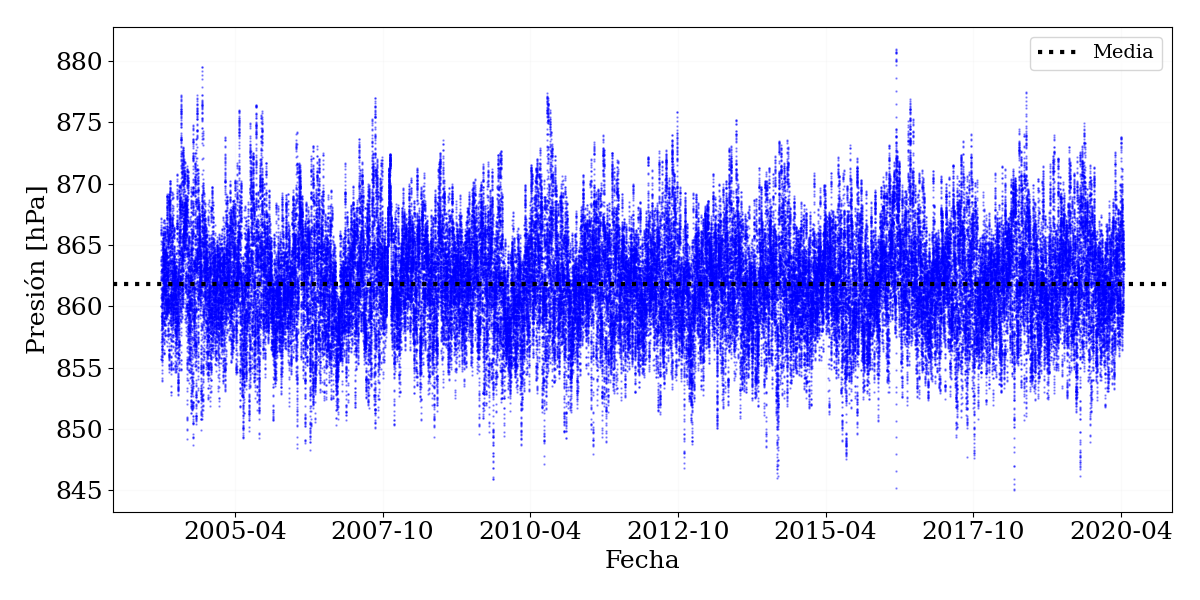
\includegraphics[width=0.8\textwidth]{Graphs/clima/presion_v2.png}
	\caption{Variación de la presión sobre el Observatorio en función del tiempo}
  \label{fig:clima_p}
\end{figure}


%|SD 1500
% \section{Resultados para el arreglo principal}
\section{Eventos asociados al Disparo Estándar en el rango 2004-2018}\label{Stan_modulacion}	
	
Para el SD 1500\,m se trabajó con los conjuntos de datos  presentados en la ICRC 2015  y  en la ICRC 2019.La señal de $S(1000)$ fue corregida en la reconstrucción oficial de eventos por la modulación del clima, por los parámetros obtenidos en \cite{aab2017impact}, mediante un análisis de los datos registrados  entre los años 2005-2015. En este trabajo se emula el análisis de datos realizado en \cite{aab2017impact} con los mismos datos, con el fin de verificar que se obtienen los mismos resultados. Luego se realizó un análisis similar con los datos de nueva reconstrucción de la señal $S_{38}$ sin la corrección del clima  del conjunto de datos de la ICRC 2019 en el periodo 2005-2018. %Posterior este análisis, se realizó un reconstrucción de la energía mediante un valor de $S_{38}$ del los datos de la ICRC 2019.% y la señal S$_{38}$ corregida por el clima S$_{38}$$_w$, para comparar resultados entre sí.

\begin{figure}[H]
	\centering
        \begin{subfigure}[b]{0.8\textwidth}	
			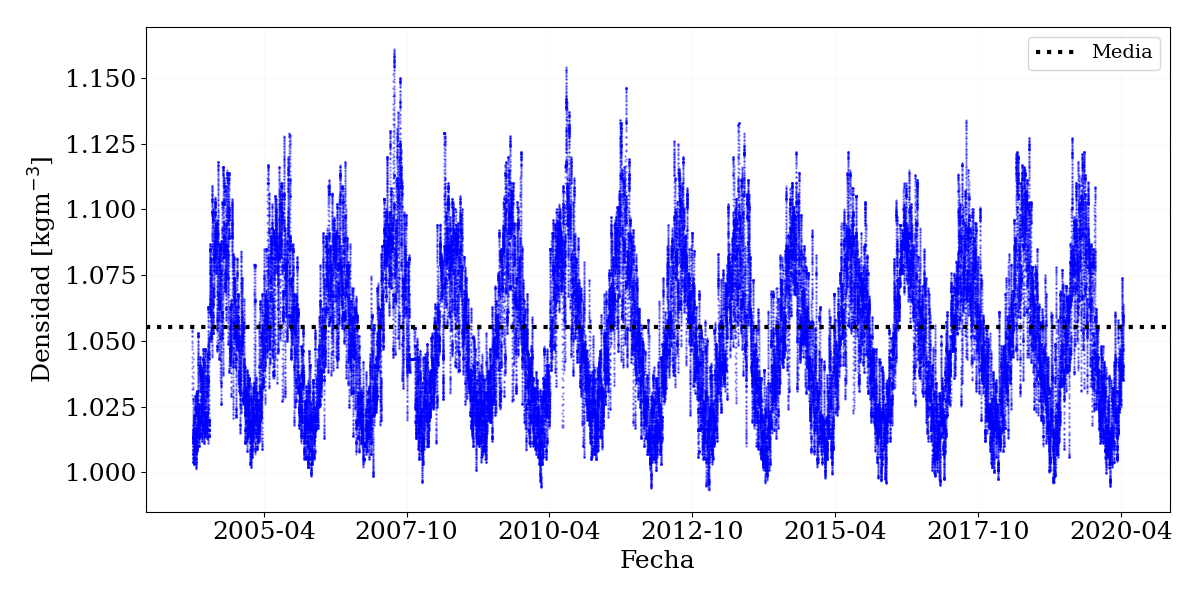
\includegraphics[width=\textwidth]{Graphs/clima/densidad_diaria_v2.png}
			\caption{Densidad diaria}
			\label{fig:densidad_diaria}
        \end{subfigure}\\
        % \hspace{\fill}
        \begin{subfigure}[b]{0.8\textwidth}
			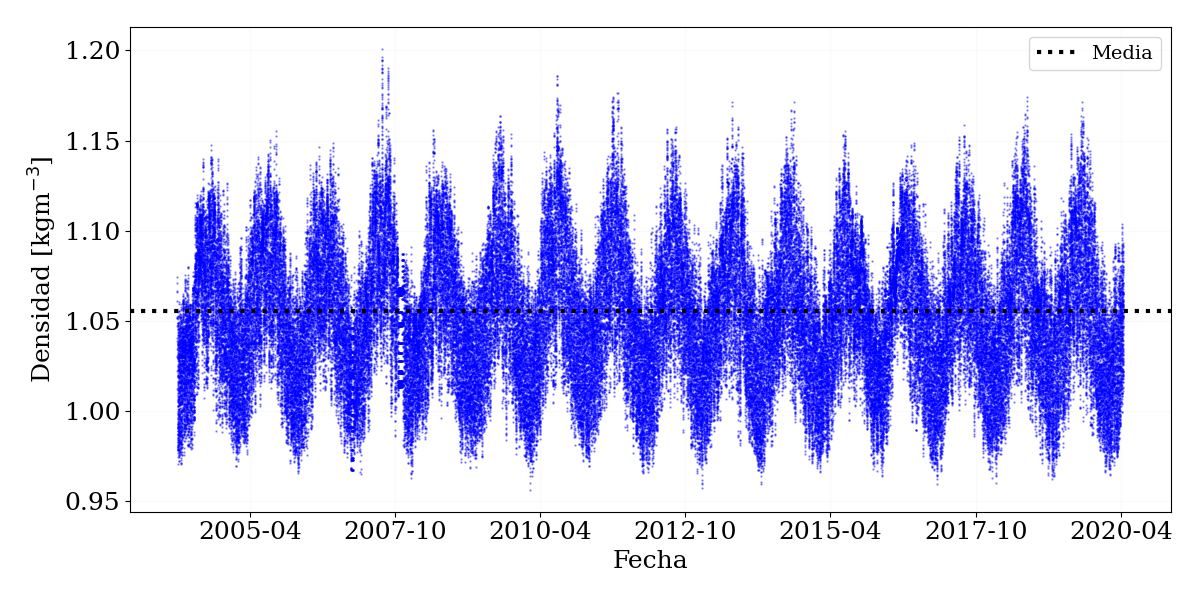
\includegraphics[width=\textwidth]{Graphs/clima/densidad_media_diaria_v2.png}
			\caption{Densidad media por hora}
			\label{fig:densidad_hora}
		\end{subfigure}\\
		% \hspace{\fill}
        \begin{subfigure}[b]{0.8\textwidth}	
			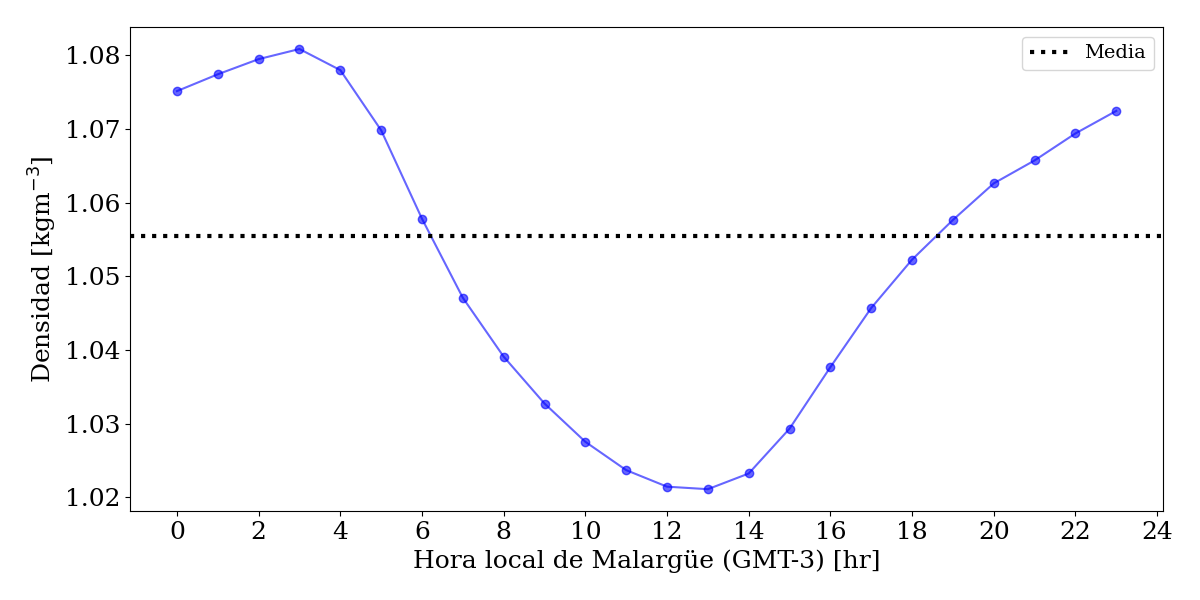
\includegraphics[width=\textwidth]{Graphs/clima/densidad_hod_v2.png}
			\caption{Densidad media por hora del día.}
			\label{fig:area_auger}
        \end{subfigure}\\
  \caption{Variaciones de las variables del clima en función del tiempo}
  \label{fig:clima_p_rho}
\end{figure}



Los coeficientes atmosféricos se obtienen tomando una energía mayor a $1\,$EeV en el caso de los datos de la ICRC 2015. Para el caso del análisis con el valor de $S_{38}$ de la ICRC 2019, se realiza el corte de eventos con el valor de $S_{38}$  que tiene un evento de $1\,$EeV. Es posible que estos coeficientes dependan de la energía, por ejemplo por la dependencia del logaritmo de la energía de $X_{max}$ o por los cambios de composición a distintas energías. En todo caso, se espera que estas dependencias sean pequeñas.% entonces los parámetros obtenidos deben describir  estos efectos. 


Para asegurarse eventos con una buena reconstrucción de  energía, posición del núcleo y dirección de arribo, solo los eventos que están contenidos dentro del arreglo del SD son considerados. Este criterio requiere que el detector con mayor señal esté rodeado de 6 tanques activos. Teniendo en cuenta la geometría de arreglo de WCDs, se calcula el área efectiva mediante la suma del área asociada a cada tanque. El mismo contribuye un área de $\sqrt{3} \frac{d^2}{2}$, donde $d$ es la distancia entre WCDs en una grilla triangular. Como la cantidad de hexágonos activos varía con el tiempo también lo hace  el área efectiva del observatorio. En la Fig.\,\ref{fig:area} se muestra la evolución del área efectiva del SD 1500 m hasta el año 2018. La línea horizontal  limita el área mínima considerada para el análisis. Estos periodos de baja exposición no proveen información suficiente para caracterizar la modulación.
Este valor de corte en el área corresponde aproximadamente al $10\%$ del valor nominal.
\begin{figure}[H]
    \centering
    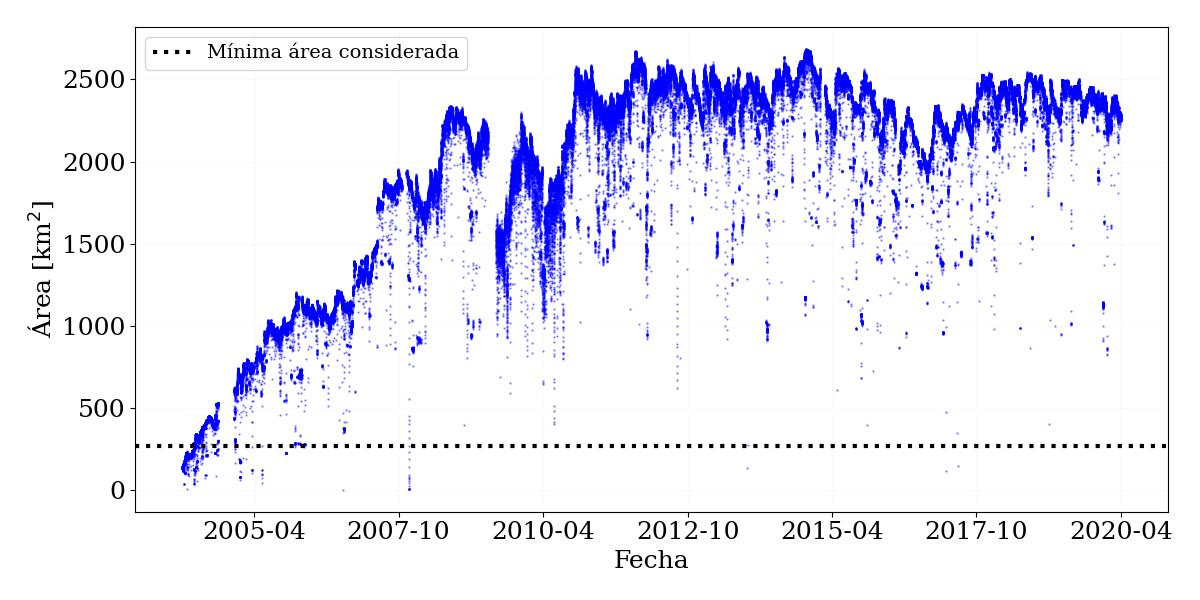
\includegraphics[width=0.9\textwidth]{Graphs/clima/area_v2.png}
    \caption{Evolución temporal del área efectiva del Observatorio Pierre Auger. La línea horizontal señala el área mínima considerada para el análisis.}
    \label{fig:area}
\end{figure}

En este trabajo se utilizan los datos recabados por las estaciones del clima del observatorio. Como se menciona en la sección \ref{seccion:clima}, existen periodos donde los datos del clima son interpolados. Es por ello que se consideran los eventos registrados durante un periodo en donde las condiciones climáticas fueron medidas o interpoladas para un periodo menor a 3 horas. % Esto se realiza para asegurar que las condiciones climáticas para un evento sean las adecuadas para realizar el análisis.

%====|==>ICRC 2015	
\subsection{Datos presentados en la ICRC 2015}\label{icrc2015}
En esta sección de utilizaron los datos de la ICRC 2015 utilizando los cortes recomendados mencionados en la sección anterior. Además de considerar eventos con energía mayor a $1\,$EeV en un periodo de tiempo entre 01/01/2005 y 31/12/2015, y con ángulo cenital $\theta$ menor que $60^o$.  Tras los cortes mencionados, se analizaron $1146470$ eventos con una la media de energía de $1.005\,$EeV. Nos referiremos a este subconjunto de datos de la ICRC 2015  como conjunto A. Las características del conjunto A se resumen en la Tabla \ref{tabla:caracteristicas_ICRC_2015}.
%====|====|	Tabla de eventos exposure
        \begin{table}[H]
            \centering
            \begin{tabular}{|c|c|}
            \hline
            \textbf{Tiempo}     & \textbf{01/01/2005-31/12/2015} \\ \hline
            %Exposición          &          							\\ \hline
            Número de eventos   &   1146470							\\ \hline 
            Energía media       &   2.00\,EeV       				\\ \hline  %  1.005\,EeV
            Corte en energía    &  1 EeV        				\\ \hline 
            Ángulo cenital		& $\theta < 60^o$ 				\\ \hline
            \end{tabular}
        \caption{Características de los datos ICRC 2015 utilizados para esta sección.} \label{tabla:caracteristicas_ICRC_2015}
        \end{table}

% ====|====|Tabla del fit
        Se realiza un ajuste de la tasa de eventos por hora del conjunto A, que incluye todos los eventos de ángulo cenital $\theta< 60^o$. Los parámetros obtenidos se presentan y se comparan con \cite{aab2017impact} en la Tabla \ref{tabla:parametros_ICRC_2015}. Los errores presentados son los errores obtenidos por el ajuste. El $\chi^2_\nu$ representa el $\chi^2$ reducido, que para este ajuste es de $\chi^2_\nu=1.01328$, por lo que el modelo propuesto representa adecuadamente los datos experimentales. Se observa que los parámetros obtenidos son compatibles con el trabajo anterior.
        \begin{table}[H]
            \centering
            \begin{tabular}{|c|c|c|}
            \hline
            \textbf{Parámetro}          & \textbf{2005-2015}            & \textbf{\cite{aab2017impact}}     \\ \hline
            $a_P$ [hPa$^{-1}$]          & $-0.0032 \pm 0.0002$          & $-0.0032 \pm 0.0003$              \\ \hline
            $a_\rho$ [kg$^{-1}$m$^3$]   & $-1.71 \pm 0.04 $             & $-1.72 \pm 0.04$                  \\ \hline
            $b_\rho$ [kg$^{-1}$m$^3$]   & $-0.51 \pm 0.05$              & $-0.53 \pm 0.04$                  \\ \hline
            $\chi^2_\nu$                & $1.01328$                     & $1.013$                         \\   \hline
            \end{tabular} 
            \caption{Ajustes obtenidos considerando todos los eventos con $\theta<60^o$ y energía mayor a $1\,$EeV, comparados con los obtenidos en \cite{aab2017impact}} \label{tabla:parametros_ICRC_2015}
        \end{table}

%====|====|	2005-2015	rate hour of the day	1 EeV
        Mediante los coeficientes obtenidos se calculó la tasa de eventos por día que predice el modelo, teniendo en cuenta los valores medios de las variables del clima para cada hora. En la Fig. \ref{fig:rate_2015_05-15} se muestra el ajuste comparado con la tasa experimental. En esta figura se observa que el modelo propuesto se corresponde con los datos experimentales, como lo indica el valor de $\chi^2_\nu=1.01328$. En la Fig.\ref{fig:rate_dayly_ICRC_2015} se muestra la tasa media por día donde la modulación anual es apreciable. Mientras que en la Fig.\ref{fig:rate_hod_ICRC_2015} se muestra el promedio por cada hora del día a partir de la tasa de eventos por hora, donde la tasa medida experimentalmente presenta una modulación diaria.  

        \begin{figure}[H]
            \centering
            \begin{subfigure}[b]{0.9\textwidth}
            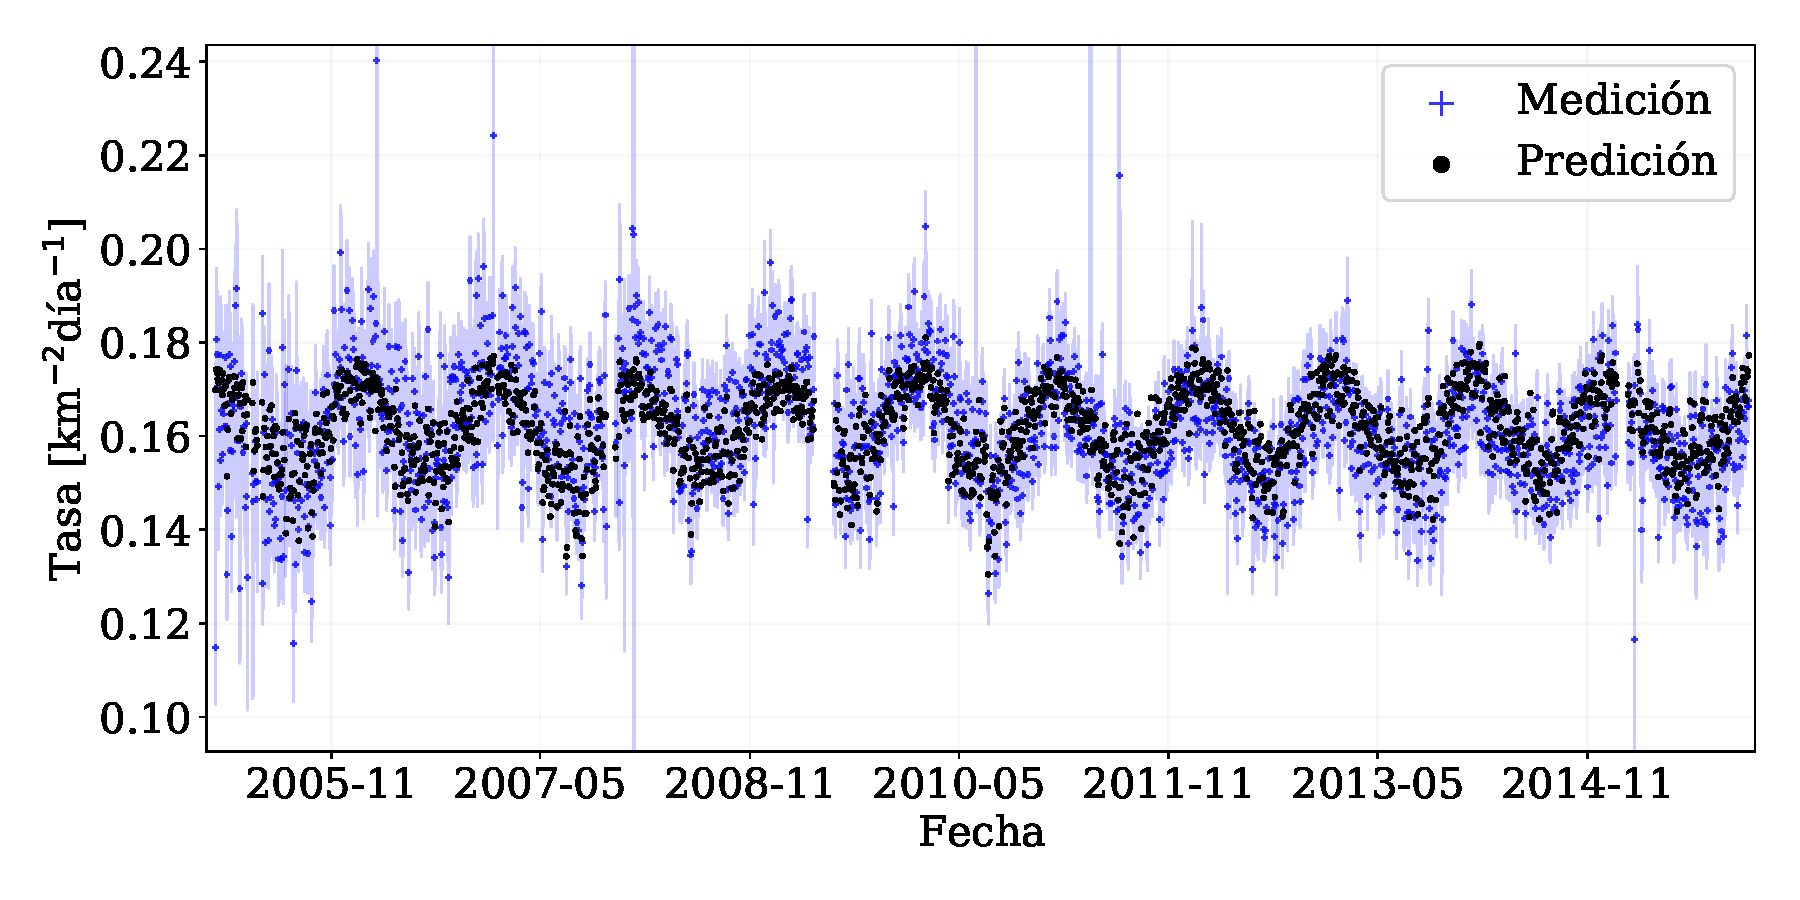
\includegraphics[width=\textwidth]{Graphs/rate_dayly/herald_old_above_1EeV_rate_day.pdf}
            \caption{Tasa eventos por día}\label{fig:rate_dayly_ICRC_2015}
            \end{subfigure}\\
            % \hspace{\fill}
            \begin{subfigure}[b]{0.9\textwidth}
            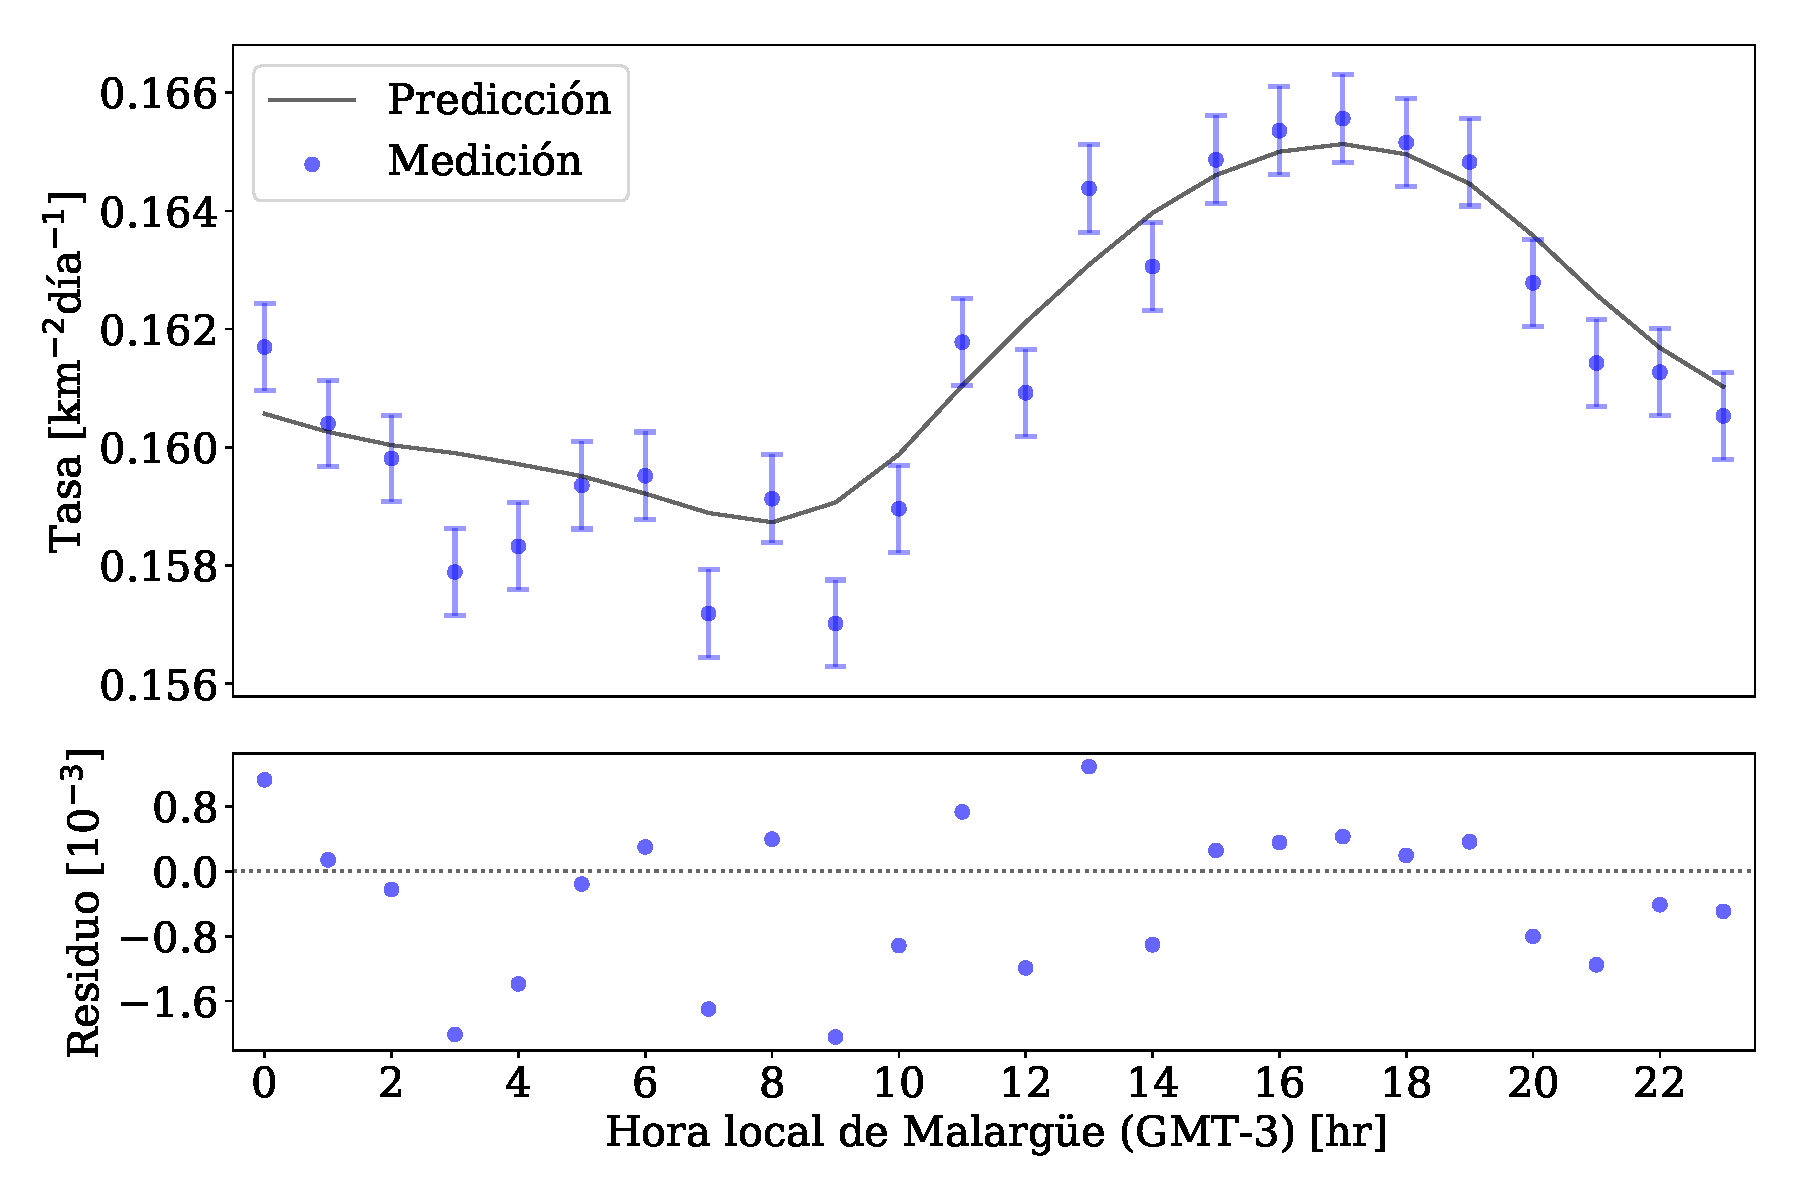
\includegraphics[width=\textwidth]{Graphs/rate_hour_of_the_day/1EeV_ICRC_2015_old_herald.pdf}
            \caption{Tasa de eventos promediada por hora del día }\label{fig:rate_hod_ICRC_2015}
            \end{subfigure}%
            \caption{Tasa de eventos por días comparadas con el ajuste entre los años 2005 hasta 2015. Los datos analizados fueron los presentados en la ICRC 2015 para energías mayores a $1\,$EeV donde se observa la modulación anual y diaria del clima. }\label{fig:rate_2015_05-15}
        \end{figure}



        \begin{figure}[H]
            \centering
            \begin{subfigure}[b]{0.5\textwidth}
            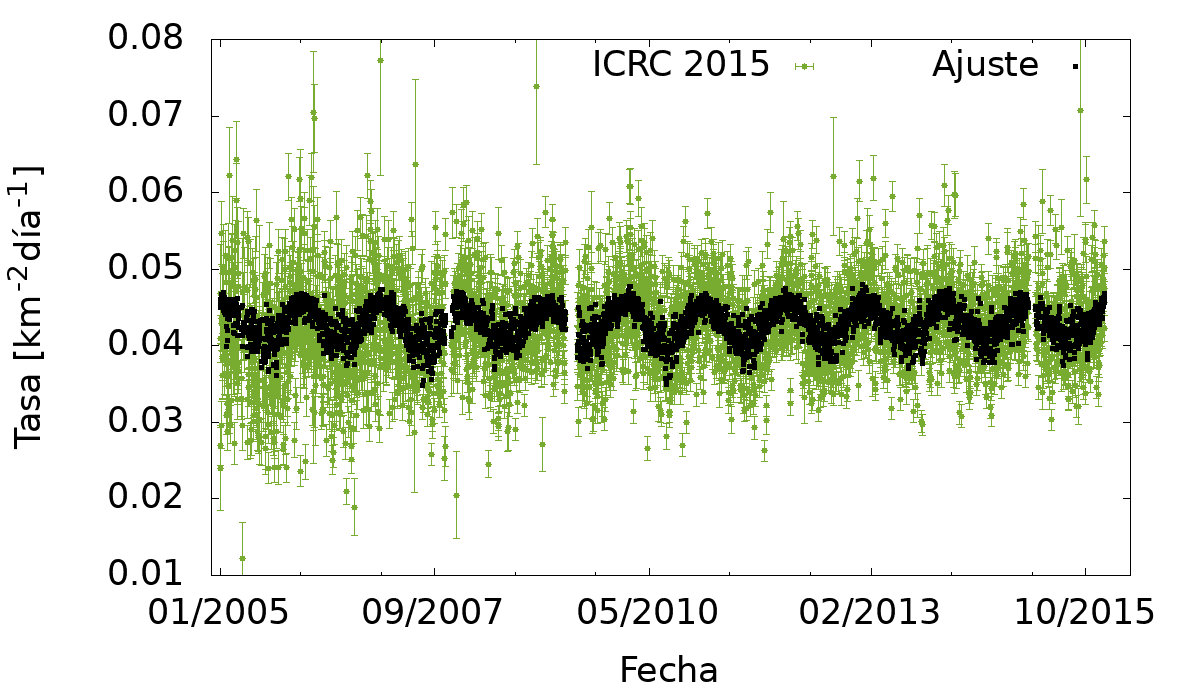
\includegraphics[width=\textwidth]{Graphs/rate_dayly/2EeV_ICRC_2015.png}
            \caption{Tasa eventos por día}\label{fig:rate_dayly_ICRC_2015_2EeV}
            \end{subfigure}\\
            % \hspace{\fill}
            \begin{subfigure}[b]{0.5\textwidth}
            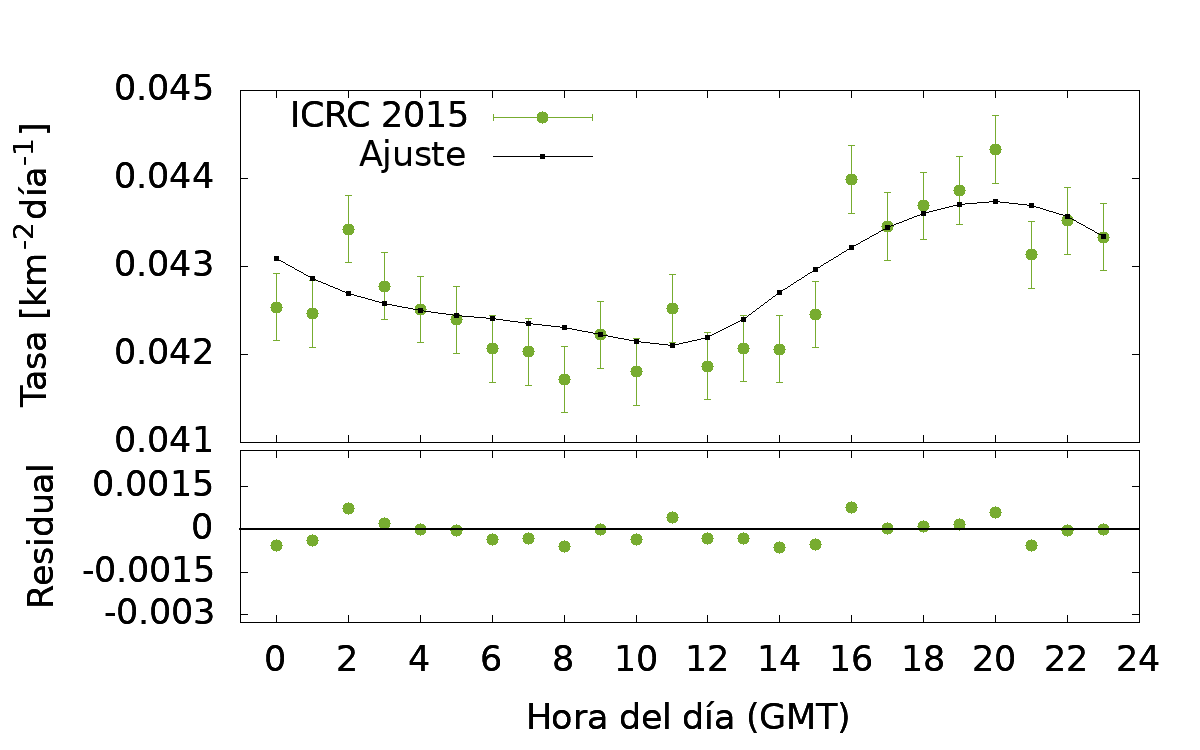
\includegraphics[width=\textwidth]{Graphs/rate_hour_of_the_day/2EeV_ICRC_2015_old_herald.png}
            \caption{Tasa de eventos promediada por hora del día }\label{fig:rate_hod_ICRC_2015_2EeV}
            \end{subfigure}%
            \caption{Tasa de eventos por días comparadas con el ajuste entre los años 2005 hasta 2015. Los datos analizados son los presentados en la ICRC 2015 para energías mayores a $2\,$EeV. donde se observa la modulación anual y diaria del clima }\label{fig:rate_2015_05-15_2EeV}
        \end{figure}

Como se menciona en la sección \ref{seccion:sd_eff}, el detector alcanza su máxima eficiencia para energías mayores que 3\,EeV. A partir una energía de $2\,$EeV, los eventos tienen una mayor susceptibilidad al disparo de tres tanques, mínimo número necesario para la reconstrucción de un evento. Para el conjunto A, como se muestra en la Fig.\,\ref{fig:rate_2015_05-15_2EeV}, la modulación del clima aún es apreciable para una energía mayor a $2\,$EeV. 
%====|====|	Weather params
        \subsubsection{Ajuste de los parámetros del clima}
        En esta sección se estudia la dependencia de los parámetros del clima con el ángulo cenital. Clasificamos los eventos en distintos subconjuntos según el valor de $sin^2(\theta)$ para realizar un ajuste análogo al presentado en la Tabla \ref{tabla:parametros_ICRC_2015}. Se clasifica mediante este valor para obtener números de eventos similares para cada subconjunto. Estos ajustes son presentados en las Figs. \ref{fig:ap_2015}, \ref{fig:arho_2015} y \ref{fig:brho_2015}. Los mismos se comparan con los datos presentados en \cite{aab2017impact}, usados actualmente en la corrección de los datos del Observatorio Pierre Auger. Se observa que los ajustes hechos sobre el conjunto A son compatibles con los ajustes realizados en  el trabajo \cite{aab2017impact}. 
%====|====|====|	ap, arho, brho 2005-2015 vs JINST over 1 EeV
                \begin{figure}[H]
                    \centering
                    \begin{subfigure}[b]{0.8\textwidth}
                    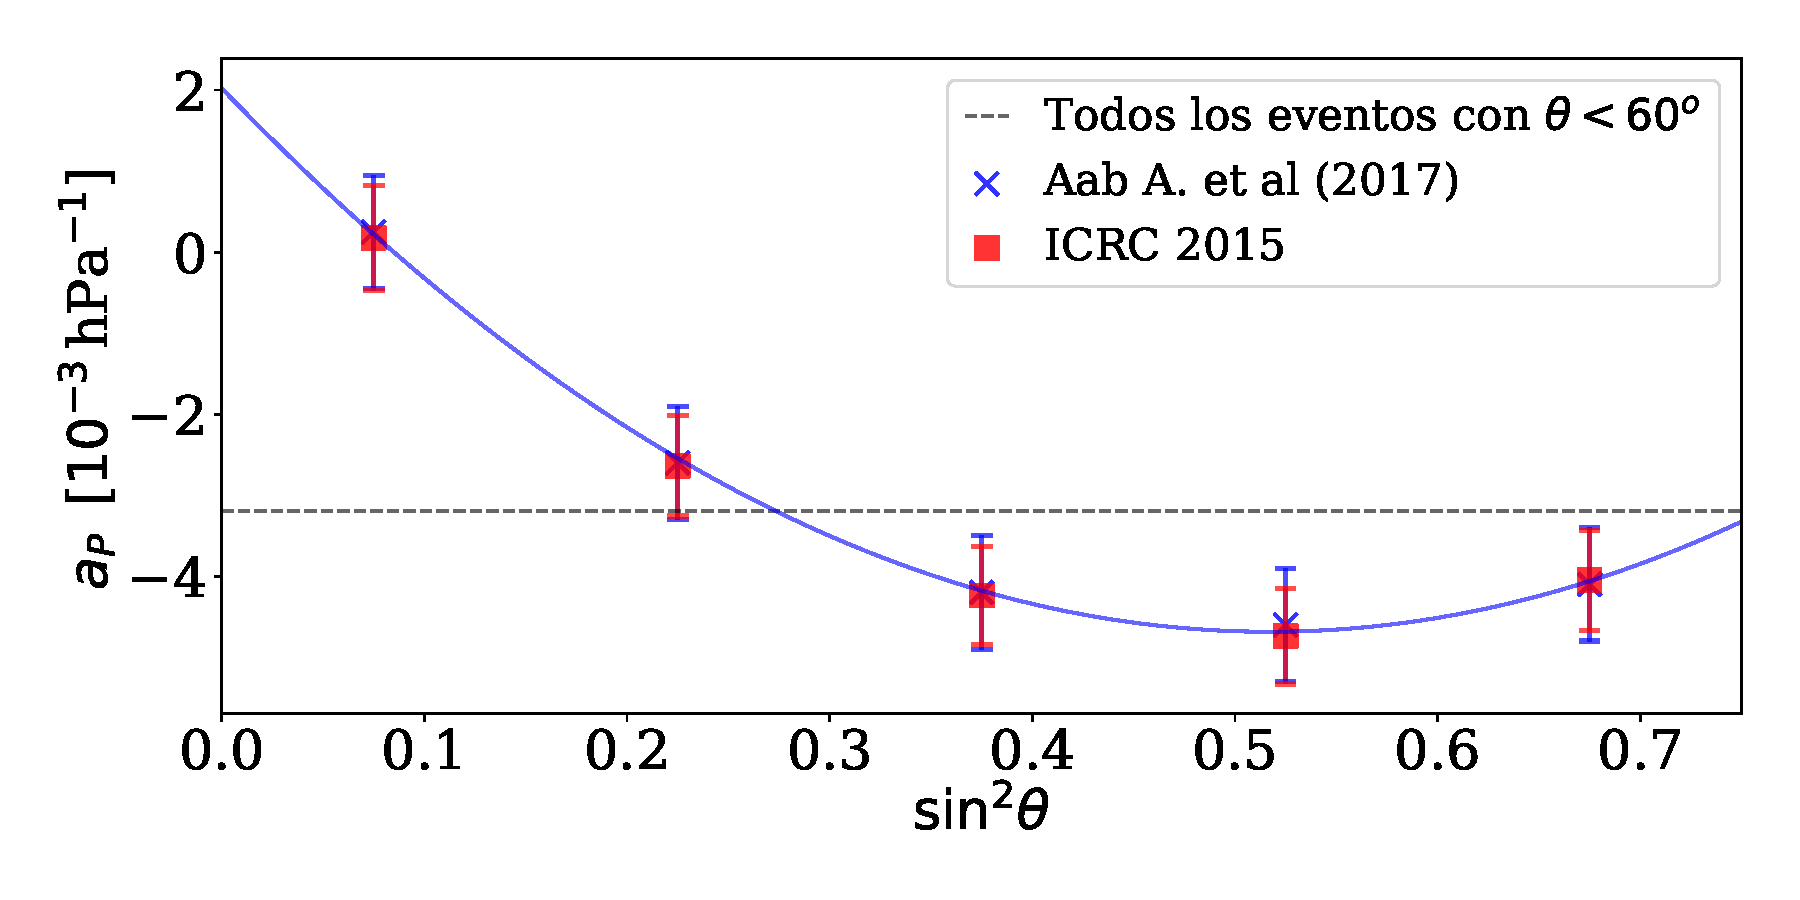
\includegraphics[width=\linewidth]{Graphs/params/ap_ICRC_2015_above_1EeV_v2.pdf}
                    \caption{Parámetro $a_P$ }
                    \label{fig:ap_2015}
                    \end{subfigure}\\
                    % \hspace{\fill}
                    \begin{subfigure}[b]{0.8\textwidth}
                    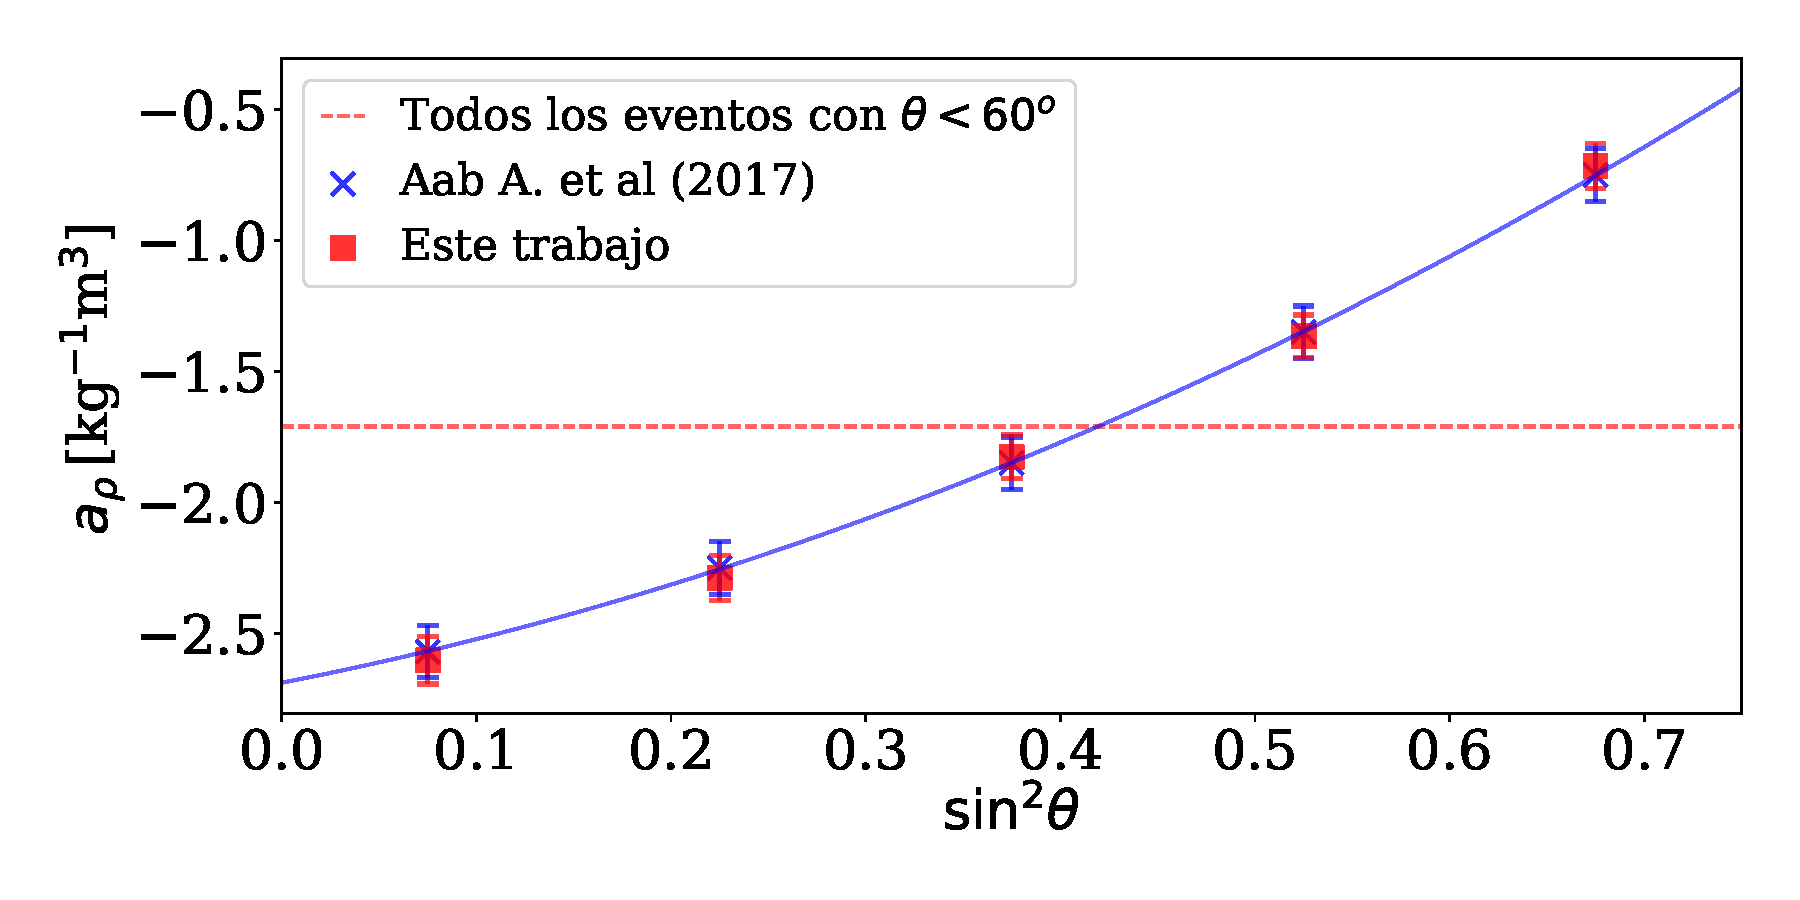
\includegraphics[width=\linewidth]{Graphs/params/arho_ICRC_2015_above_1EeV_v2.pdf}
                    \caption{Parámetro $a_{\rho}$ }
                    \label{fig:arho_2015}
                    \end{subfigure}\\
                    % \hspace{\fill}
                    \begin{subfigure}[b]{\textwidth}
                    \centering
                    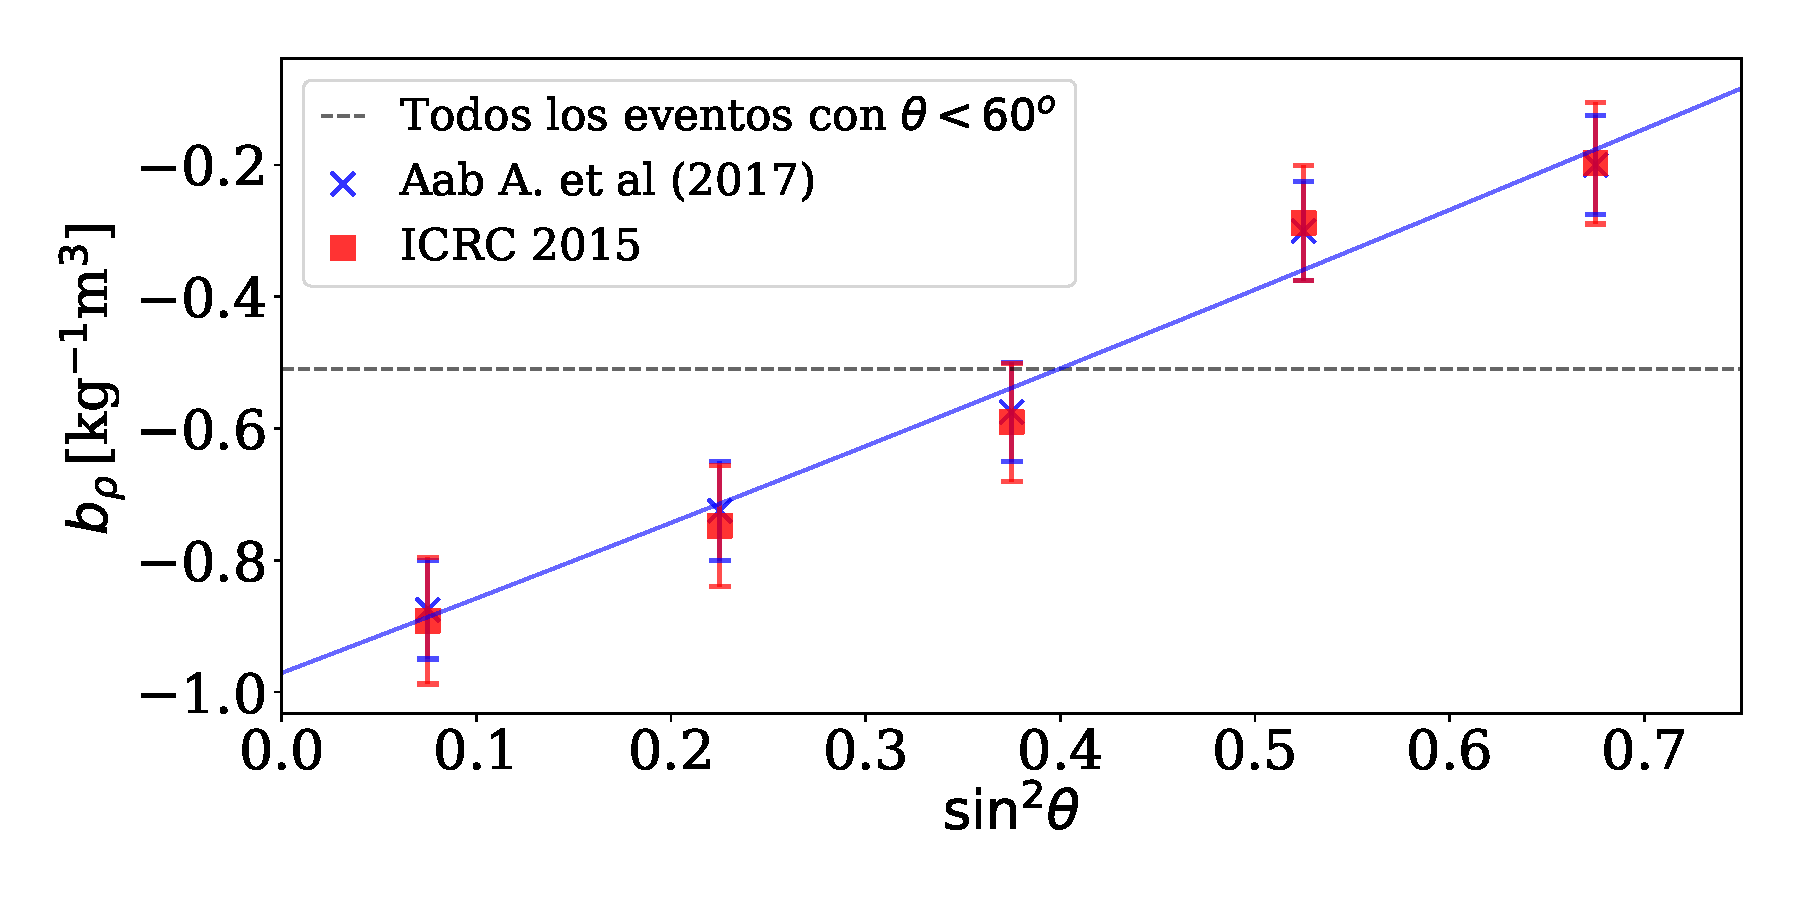
\includegraphics[width=0.8\linewidth]{Graphs/params/brho_ICRC_2015_above_1EeV_v2.pdf}
                    \caption{Parámetro  $b_{\rho}$	 }
                    \label{fig:brho_2015}
                    \end{subfigure}%
                    \caption{Parámetros de la modulación del clima considerando los datos de la ICRC 2015. Los mismos se comparan con los ajustes obtenidos en \cite{aab2017impact} y con los ajustes obtenidos sin considerar la dependencia con $sin^2(\theta)$. }\label{fig:parameters_old}
                \end{figure}
%====|====|====| 	Tabla de c0, c1, c2
            En la Fig. \ref{fig:parameters_old} también se compara los ajustes obtenidos considerando los datos sin clasificar por $sin^2\theta$. Se observa que existe una dependencia con el ángulo cenital correspondiente al evento. Esta dependencia fue modelada mediante una función cuadrática dada en la Ec.\,\ref{eq:cuadratica}
            \begin{equation}
                f(x) = c_0 + c_1x + c_2x^2
                \label{eq:cuadratica}
            \end{equation}
            donde $x=sin^2\theta$.  En la Tabla\,\ref{tabla:cuadratica_ICRC_2015} se comparan los coeficientes obtenidos considerando la Ec.\,\ref{eq:cuadratica} con los mismos coeficiente obtenidos en el trabajo anterior \cite{aab2017impact}. 

        La dependencia con el ángulo cenital se debe a que para distintos ángulos de incidencia la lluvia interactúa con más o menos atmósfera. Los efectos de las condiciones climáticas afectan el desarrollo de la lluvia. Por ejemplo, el coeficiente de la presión  es negativo para $\sin^2(\theta)>0.3$ o $\theta>33^o$, lo que indica que si presión sube la señal baja. Esto es una consecuencia de que la lluvia  está en un estado más avanzado de su desarrollo. Para ángulos cenitales cercanos a $60^o$, la componente electromagnética es suprimida por las interacciones en la atmósfera, por lo tanto el efecto de la presión disminuye. El resultado obtenido en la Fig.\,\ref{fig:ap_2015} es consistente con este fenómeno, dado que el valor de $a_P$ disminuye al aumentar el ángulo. 		En el caso de los coeficientes relacionados con la densidad, también se observa que los parámetros son negativos, dado que un aumento de la densidad disminuye $r_M$ y por lo tanto la extensión de la señal. Se observa también que los parámetros $a_\rho$ y $b_\rho$ tienen la misma tendencia con $\sin^2(\theta)$, además de que los coeficientes tienen una razón de aproximadamente $\nicefrac{1}{3}$, lo cual se esperaba por lo discutido en la sección \ref{seccion:fisica_clima}.
                \begin{table}[H]
                    \centering
                    \begin{tabular}{|l|l|l|l|}\hline
                         Parámetros									& Coeficiente		& Este Trabajo			& \cite{aab2017impact}	\\ \hline
                     \multirow{3}{*}{$a_P$ [hPa$^{-1}$]}  			&  $c_0$			& $ 0.00200\pm 0.00005$	& $0.0021 \pm 0.0009 $	\\ \cline{2-4} %Done
                                                                     &  $c_1$			& $-0.0263 \pm 0.0002$	& $-0.026 \pm 0.006 $	\\ \cline{2-4} 
                                                                    &  $c_2$			& $ 0.0257 \pm 0.0002$	& $0.026  \pm 0.007 $	\\ \hline % 
                    
                     \multirow{3}{*}{$a_\rho$ [kg$^{-1}$m$^3$]}  	&  $c_0$			& $-2.73   \pm 0.05$	& $ -2.7  \pm 0.1  $\\ \cline{2-4} 
                                                                     &  $c_1$			& $ 1.5    \pm 0.4 $	& $ 1.5   \pm 0.8  $\\ \cline{2-4} 
                                                                    &  $c_2$			& $ 2.1    \pm 0.7 $	& $ 2.2   \pm 1.0  $\\ \hline %
                    
                    \multirow{3}{*}{$b_\rho$ [kg$^{-1}$m$^3$]} 		&  $c_0$			& $-1.0    \pm 0.1$		& $-1.0   \pm 0.1 $	\\ \cline{2-4} 
                                                                    &  $c_1$			& $ 1.2    \pm 0.6$		& $ 1.2   \pm 0.8  $	\\ \cline{2-4} 
                                                                    &  $c_2$			& $ 0.1    \pm 0.8$		& $ 0.0   \pm 1.1  $	\\ \hline 
                    
                    \end{tabular}	
                    \caption{Tabla de los coeficientes obtenidos para el conjunto de datos de la ICRC 2015, comparados con el trabajo anterior \cite{aab2017impact}} \label{tabla:cuadratica_ICRC_2015}
                \end{table}

%==================================================================================================================
%==================================================================================================================
%==================================================================================================================
%==================================================================================================================

%====|==> ICRC 2019
 \subsection{Datos presentados en la ICRC 2019}\label{conjuntoB}
     Comparando este conjunto de datos con los datos de la ICRC 2015, los datos de la ICRC 2019 contienen eventos de los tres años posteriores. Posterior al trabajo \cite{aab2017impact}, la señal de S(1000) fue corregida por las condiciones climáticas en la reconstrucción oficial de eventos. Además el valor de S(1000) estimado para cada evento cambió entre estos dos conjuntos de datos, por parte de la reconstrucción oficial \cite{isabel}. Se realizó también una nueva calibración de la energía mediante eventos híbridos, como la mostrada en la Fig.\,\ref{fig:efd_s38} en el trabajo  \cite{tobepublished}. En el conjunto de datos de la ICRC 2019, se realizó los mismos cortes que para el conjunto de A de la sección anterior. En el periodo 2005-2015 de los datos de la ICRC 2019 con los cortes mencionados de energía mayor a $1\,$EeV para eventos verticales, la cantidad de eventos con energías mayores a $1\,$EeV subió de 1146470 a  1280918 eventos. Esto puede deberse a la corrección del clima de los eventos, donde aquellos eventos que estaban por debajo del corte del energía, tras la corrección pudieron estar por encima de este corte. Otro posibilidad es la nueva reconstrucción haya aumentado la cantidad de eventos por encima de $1\,$EeV. Por eso la media de energía bajó de $2.00\,$EeV a $1.91\,$EeV.  Las características de los datos en estos dos rangos de tiempo se resumen en la Tabla\,\ref{tabla:caracteristicas_ICRC_2019}. 
%====|====|	Tabla de eventos exposure
        \begin{table}[H]
            \centering
            \begin{tabular}{|c|c|c|}
            \hline
            \textbf{Tiempo }    & \textbf{01/01/2005-31/12/2015}  & \textbf{01/01/2005-31/12/2018 }\\ \hline 
            %Exposición          &          				 &          			\\ \hline
            Número de eventos   &  1280918     			 &  1635045     		 \\ \hline 
            Energía media       &  1.91				 &	1.92				\\ \hline % 1.0734        		 &  1.1370       			\\ \hline 
            Corte en energía    &  1 EeV       		 	 &  1 EeV       		 \\ \hline 
            Ángulo cenitales	&  $60^o$ 				 & $60^o$\\ \hline
            \end{tabular}
            \caption{Características de los datos de la ICRC 2019 utilizados para los ajustes de esta sección.} \label{tabla:caracteristicas_ICRC_2019}
        \end{table}

        En la Fig.\,\ref{fig:rate_new_18} se muestran las tasas de eventos por día para energía mayores a $1\,$EeV y $2\,$EeV, con la energía corregida por los efectos climáticos según la reconstrucción oficial \cite{data}. En la Fig.\,\ref{fig:rate_new_18_2EeV} se  comparan con los resultados de los datos de la ICRC 2015, la modulación en la tasa ya no es apreciable. Si comparamos las tasas de eventos por hora del día de los eventos por encima de $1\,$EeV y $2\,$EeV, por encima de $1\,$EeV, se aprecia un remanente de la modulación del clima diaria comparado con la tasa para $2\,$EeV. Esto se debe a que el SD tiene eficiencia para energía mayores a $3\,$EeV, comentado anteriormente.


            Existe una modulación remanente en la tasa de eventos como se aprecia en las Figs.\,\ref{fig:rate_day_ICRC_19_05_18} y \ref{fig:rate_day_ICRC_19_05_18_2EeV}. Esto se debe que la señal es mayor que la esperada como consecuencia de las condiciones atmosféricas en el momento del evento, por lo tanto la eficiencia del disparo ante este evento también es mayor. De esta forma la eficiencia tiene una dependencia con las condiciones atmosféricas.
%====|====|	2005-2019	rate day over 1 EeV
%====|====|	2005-2019	rate hour of the day	1 EeV
        \begin{figure}[H]
            \centering
            \begin{subfigure}[b]{0.5\textwidth}
            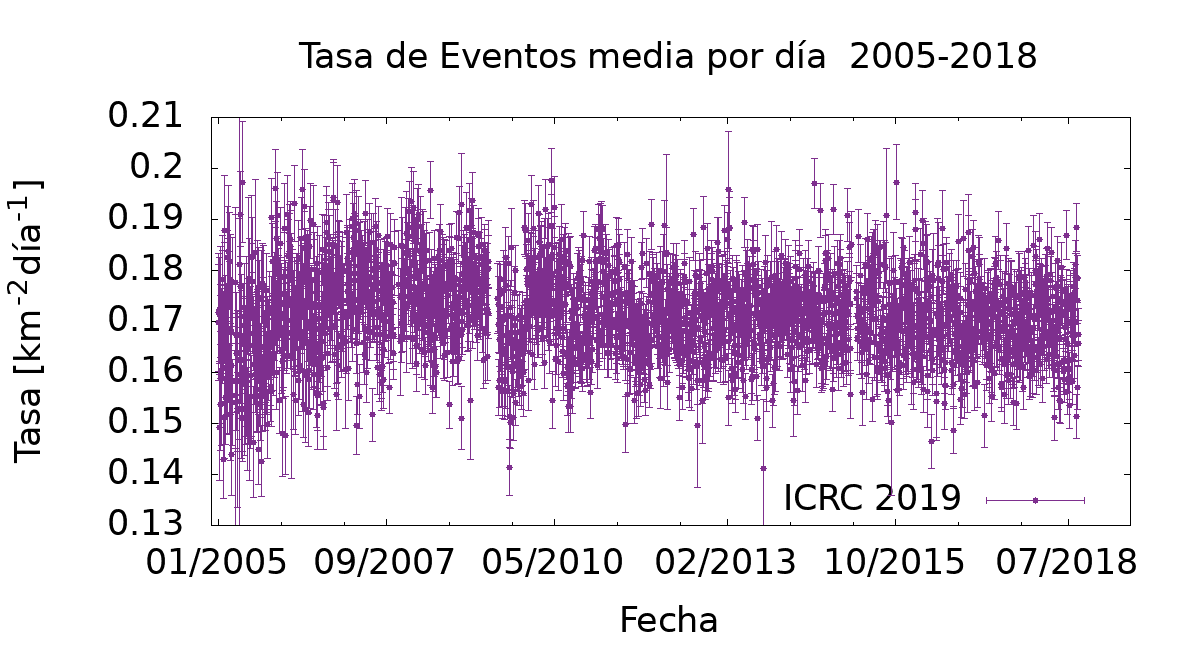
\includegraphics[width=\textwidth]{Graphs/rate_dayly/1EeV_ICRC_2019_05_18.png}
            \caption{Energía mayor a $1\,$EeV}
            \label{fig:rate_day_ICRC_19_05_18}
            \end{subfigure}\\
            % \hspace{\fill}
            \begin{subfigure}[b]{0.5\textwidth}
            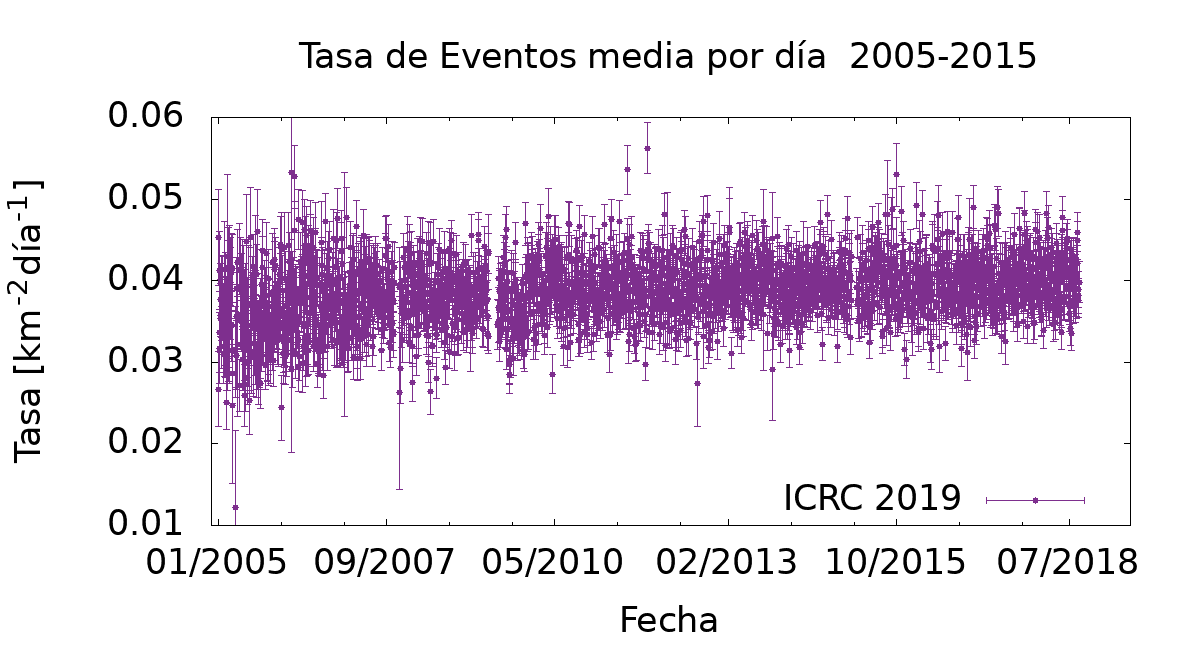
\includegraphics[width=\textwidth]{Graphs/rate_dayly/2EeV_ICRC_2019_05_19.png}
            \caption{ Energía mayor a $2\,$EeV}
            \label{fig:rate_2015_ICRC_19_05_18}
            \end{subfigure}%
            \caption{Tasa de eventos promedio por cada día entre los años 2005 hasta 2015 del conjunto de datos presentado en la ICRC 2019. Se muestran las tasas para dos cortes en energía, mayor a $1\,$EeV y mayor a $2\,$EeV}\label{fig:rate_new_18}
        \end{figure}
        \begin{figure}[H]
            \centering
            \begin{subfigure}[b]{0.495\textwidth}
            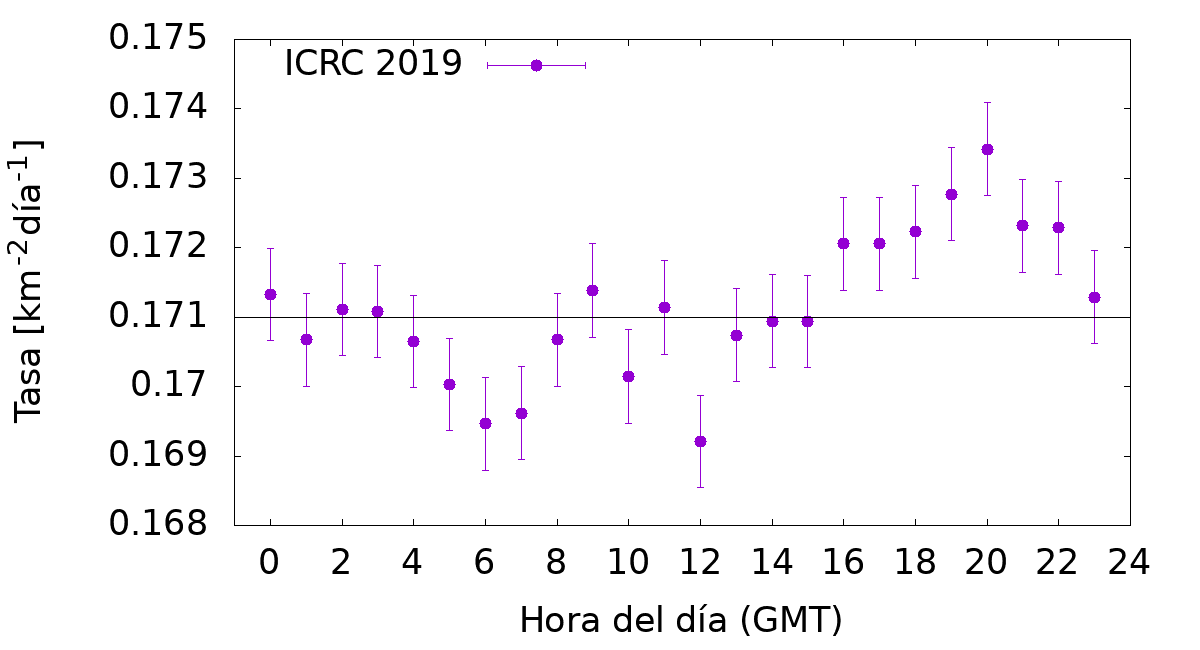
\includegraphics[width=\textwidth]{Graphs/rate_hour_of_the_day/1EeV_ICRC_2019_05_19.png}
            \caption{Energía mayor a $1\,$EeV}
            \label{fig:rate_day_ICRC_19_05_18_2EeV}
            \end{subfigure}\\
            % \hspace{\fill}
            \centering
            \begin{subfigure}[b]{0.495\textwidth}
            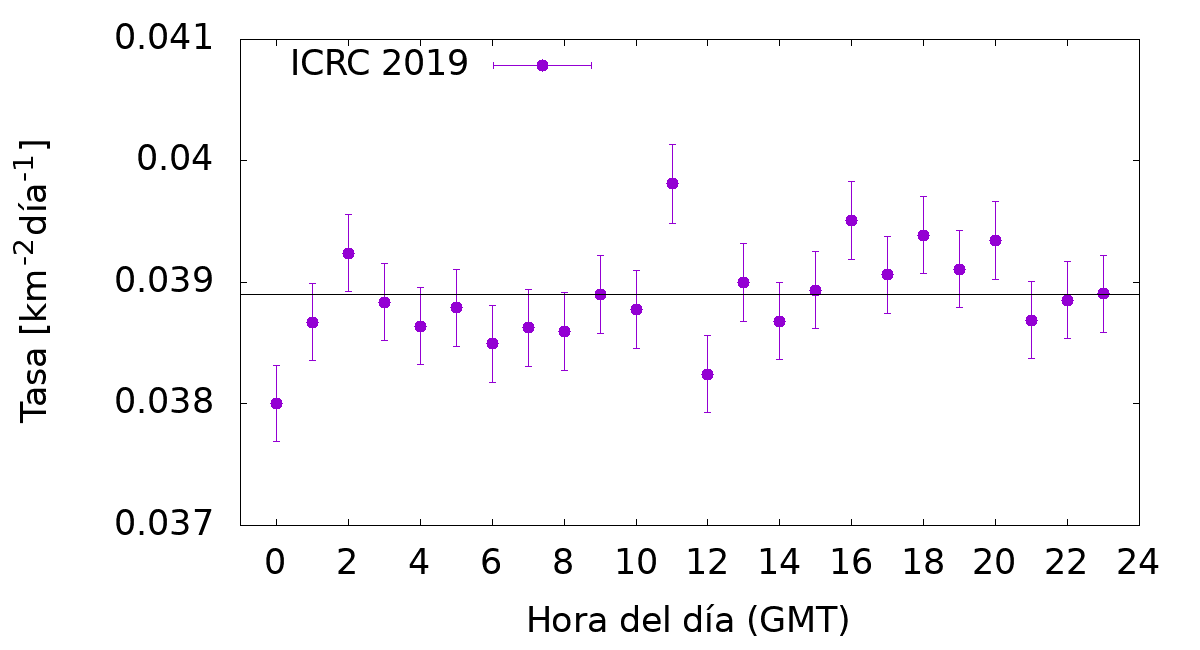
\includegraphics[width=\textwidth]{Graphs/rate_hour_of_the_day/2EeV_ICRC_2019_05_18.png}
            \caption{Energía mayor a $2\,$EeV}
            \label{fig:rate_2015_ICRC_19_05_18_2EeV}
            \end{subfigure}%
            \caption{Tasa eventos  por hora del día por unidad de área entre los años 2005 hasta 2015 del conjunto de datos presentado en la ICRC 2019.  Se muestran las tasas para dos cortes en energía, mayor a $1\,$EeV y mayor a $2\,$EeV}\label{fig:rate_new_18_2EeV}
        \end{figure}



%====|==>ICRC 2019 S$_{38}$-Sin Corrección
\subsection{Datos presentados en la ICRC 2019 usando $S_{38}$ sin corregir por el clima}

Además de tener más estadística de los eventos registrados, durante el periodo 2016-2018 también se recabaron datos sobre el clima en el observatorio. La modulación del clima fue estudiada anteriormente realizando un corte de la energía sin corregir. En esta sección se realiza el análisis de la modulación mediante un  corte sobre la señal medida por el SD. En el conjunto de datos de la ICRC 2019, es posible acceder al valor de S(1000) sin corregir por el trabajo \cite{aab2017impact}, por que uno puede obtener el valor de S$_{38}$ sin corregir mediante la expresión
\begin{equation}
    S_{38} = \frac{S(1000)}{S(1000)_w}S_{38,w}
    \label{eq:s38_w}
\end{equation}
donde las variables $S(1000)_w$ y $S_{38,w}$ indican los valores corregidos por clima. Estas variables están listadas en el conjunto de datos presentado en la ICRC 2019. Dado que los trabajos anteriores se basaron en la energía para hacer el corte de los eventos, se realizó el corte con la señal de $S_{38}\ge 5.37\,$VEM correspondiente a 1\,EeV aproximadamente. %Mediante este corte, el análisis no tiene en cuenta las correcciones del clima y es posible obtener parámetros del clima mediante el valor de S$_{38}$. 
Las características de este conjunto de datos están resumidos en la Tabla\,\ref{tabla:caracteristicas_ICRC_2019_S38}.
%====|====|	Tabla de eventos exposure
        \begin{table}[H]
            \centering
            \begin{tabular}{|c|c|c|}
            \hline
            \textbf{Tiempo }    & \textbf{01/01/2005-31/12/2015}  & \textbf{01/01/2005-31/12/2018 }\\ \hline 
            %Exposición          &          				 &          			\\ \hline
            Número de eventos   &   1267265     		 &  1618717     		\\ \hline 
            Energía media       &  1.89        		 	 &  1.90        		\\ \hline 
            Corte en S$_{38}$ 	    &  5.37\,VEM   		 	 &  5.37\,VEM       	\\ \hline 
            Ángulo cenital 		&  $<60^o$ 			 	 & $<60^o$\\ \hline
            \end{tabular}
            \caption{Características de los datos de la ICRC 2019 utilizados para los ajustes de esta sección.} \label{tabla:caracteristicas_ICRC_2019_S38}
        \end{table}

        %Cabe destacar que la cantidad de eventos considerados para el periodo 2005-2015 para este caso es mayor que para la ICRC 2015 en el mismo periodo. Esto se debe que tras la corrección del clima para la ICRC 2019, las energías cambiaron ligeramente, por lo que se tiene en cuenta eventos con energía reconstruida, menor a  1 EeV. Esto se aprecia en la disminución de la energía media.
        
%====|====| Tabla del fit
        Con estos eventos, se realizó un  ajuste de los parámetros del clima para todos los ángulos cenitales de la tasa del eventos por hora. Así se obtienen los coeficientes promediados por ángulo cenital. Estos parámetros son presentados en la Tabla\,\ref{tabla:parametros_ICRC_2019_S38}. Se observa que para ambos periodos estudiados los parámetros obtenidos son compatibles entre sí, además de ser compatibles con los resultados obtenidos para el periodo 2005-2015 de los datos de la ICRC 2015 y los parámetros de \cite{aab2017impact}, presentados en la Tabla\,\ref{tabla:parametros_ICRC_2015}.

        \begin{table}[H]
            \centering
            \begin{tabular}{|c|c|c|}
            \hline
            \textbf{Parámetro}          & \textbf{2005-2015}    		& \textbf{2005-2018}    \\ \hline
            $a_P$ [hPa$^{-1}$]          & $ -0.0033\pm 0.0003$      	& $ -0.0032\pm 0.0002$  \\ \hline
            $a_\rho$ [kg$^{-1}$m$^3$]   & $ -1.75\pm 0.04$            	& $ -1.71\pm 0.03$       \\ \hline
            $b_\rho$ [kg$^{-1}$m$^3$]   & $ -0.51\pm 0.04$             	& $ -0.52\pm 0.03$       \\ \hline
            $\chi^2_\nu$                & $1.00616$                     & $1.01819$              \\   \hline
            \end{tabular} 
            \caption{Parámetros del clima obtenidos para todos los ángulos cenitales para los dos rangos de tiempo estudiados.} \label{tabla:parametros_ICRC_2019_S38}
        \end{table}
        
        Calculando la tasa de eventos esperado con los parámetros de la Tabla\,\ref{tabla:parametros_ICRC_2019_S38}, esta se comparan con la tasa experimental medida con el SD, que se muestra en la Fig. \ref{fig:rate_new_18_S38} para el rango de tiempo 2005-2018. En estos gráficos se observa que la modulación del clima tiene la mismas características que las observadas en la sección \ref{icrc2015}.

        \begin{figure}[H]
            \begin{subfigure}[b]{0.5\textwidth}
            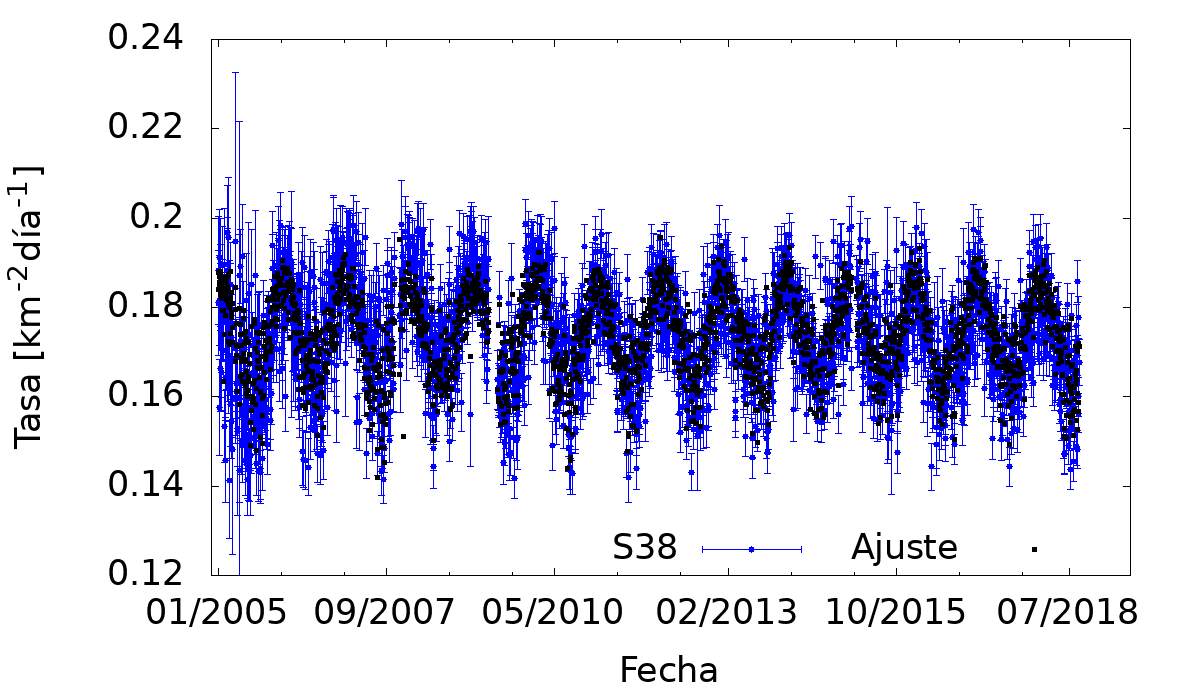
\includegraphics[width=\textwidth]{Graphs/rate_dayly/0EeV_ICRC_2019_S38_05_18.png}
            \caption{Tasa eventos por cada día por unidad de área}
            \label{fig:rate_day_ICRC_19_S38_05_18}
            \end{subfigure}%
            \hspace{\fill}
            \begin{subfigure}[b]{0.5\textwidth}
            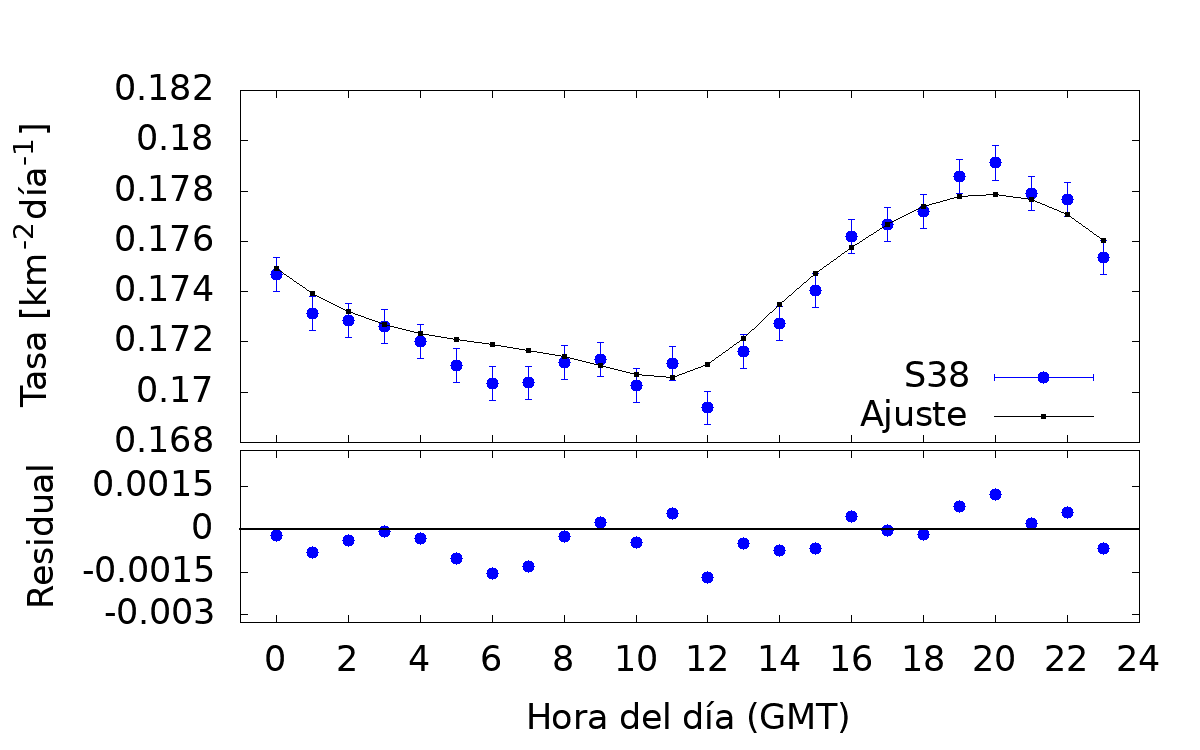
\includegraphics[width=\textwidth]{Graphs/rate_hour_of_the_day/0EeV_ICRC_2019_S38_05_18.png}
            \caption{Tasa de eventos promedio por hora del día}
            \label{fig:rate_2015_ICRC_19_S38_05_18}
            \end{subfigure}%
            \caption{Tasa de eventos entre los años 2005 hasta 2018 del conjunto de datos presentado en la ICRC 2019.}\label{fig:rate_new_18_S38}
        \end{figure}

%====|====|	Weather params
    \subsubsection{Ajuste de los parámetros del clima}
    Se clasificó los eventos de esta sección mediante el valor de $sin^2\theta$ y se realizó el ajuste para obtener los parámetros del clima. Este ajuste se realizó en el periodo 2005-2018. Los valores obtenidos se resumen en la Tabla\,\ref{tabla:cuadratica_ICRC_2019_S38} y se  observan en la Fig.\,\ref{fig:parameters_new_S38}. Comparando estos resultados con los resultados de \cite{aab2017impact}, los eventos mediante el valor S$_{38}$  conservan la tendencia con $sin^2\theta$ que se observa en los datos de la ICRC 2015 en la Fig.\,\ref{fig:parameters_old}. Además los parámetros obtenidos mediante el corte por S$_{38}$ son comparables con los resultados obtenidos para el conjunto de datos de la ICRC 2015. Por lo que puede decirse que la modulación del clima es apreciable  hasta el día de hoy con una amplitud comparable al año 2015.
%====|====|====| ap, arho, brho 2005-2015  2005-2019 vs JINST over 1 EeV
            \begin{figure}[H]
                \begin{subfigure}[b]{0.5\textwidth}
                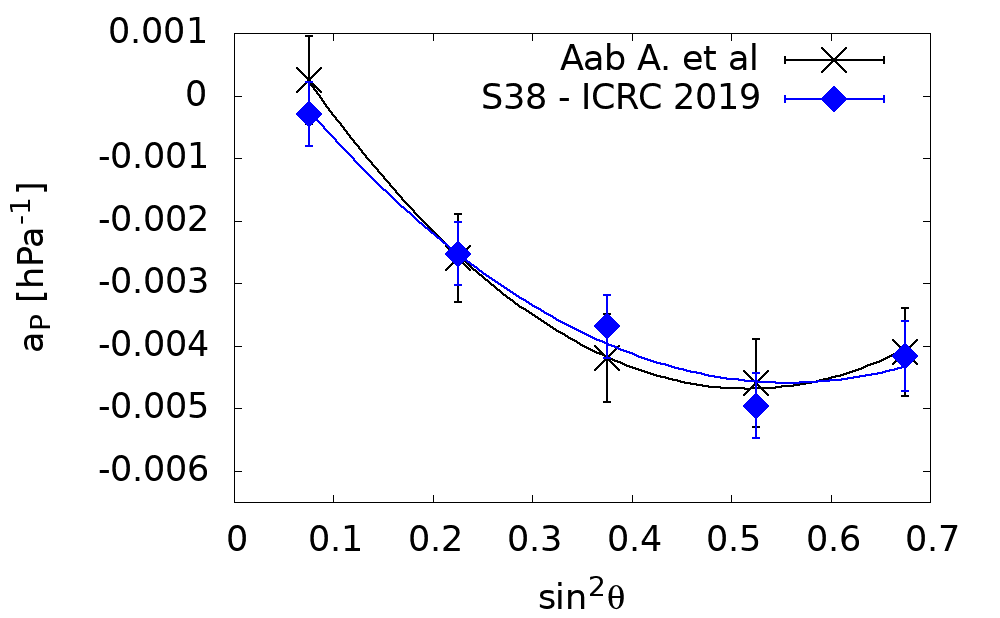
\includegraphics[width=\linewidth]{Graphs/params/ap_ICRC_2019_S38_above_0EeV.png}
                \caption{Parámetro $a_P$ }
                \label{fig:ap_2019_S38}
                \end{subfigure}%
                \hspace{\fill}
                \begin{subfigure}[b]{0.5\textwidth}
                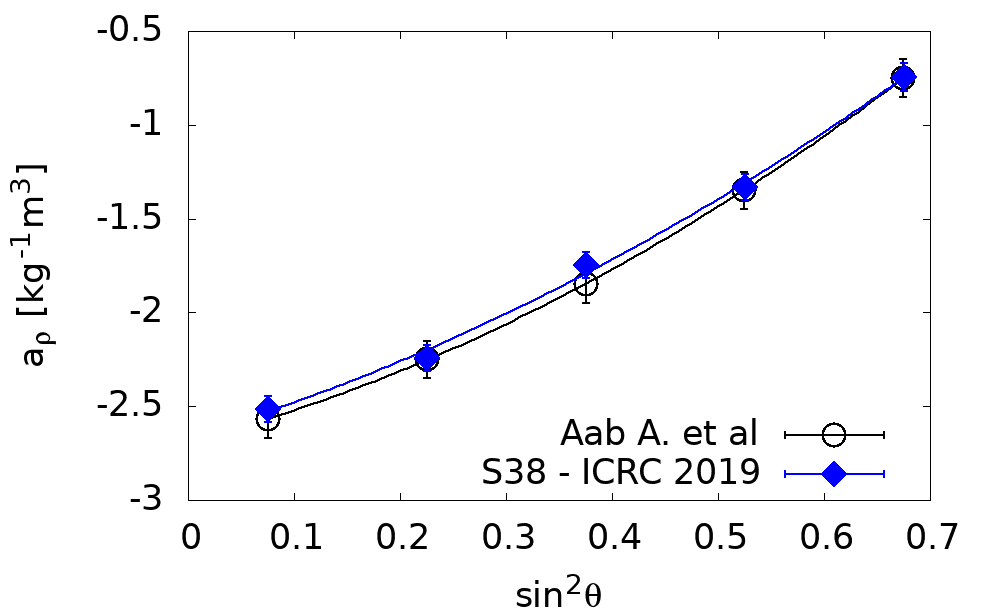
\includegraphics[width=\linewidth]{Graphs/params/arho_ICRC_2019_S38_above_0EeV.png}
                \caption{Parámetro $a_{\rho}$ }
                \label{fig:arho_2019_S38}
                \end{subfigure}%
                \hspace{\fill}
                \begin{subfigure}[b]{\textwidth}
                \centering
                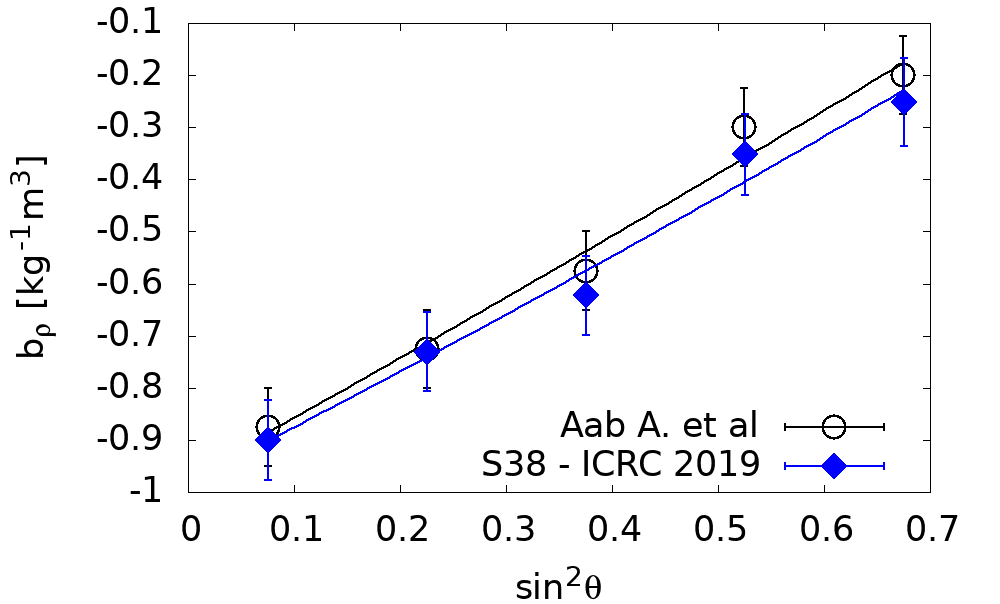
\includegraphics[width=0.5\linewidth]{Graphs/params/brho_ICRC_2019_S38_above_0EeV.png}
                \caption{Parámetro  $b_{\rho}$	 }
                \label{fig:brho_2019_S38}
                \end{subfigure}%
                \caption{Parámetros de la modulación del clima considerando los datos sin corregir con el clima y la reconstrucción anterior.}\label{fig:parameters_new_S38}
            \end{figure}
%====|====|====| Tabla de c0, c1, c2
                \begin{table}[H]
                    \centering
                    \begin{tabular}{|l|l|l|l|}\hline
                     \textbf{Parámetros}						& \textbf{Coeficiente}	& \textbf{Este Trabajo} & Reportado por \textbf{ \cite{aab2017impact}}	\\ \hline
                     \multirow{3}{*}{$a_P$ [hPa$^{-1}$]}  		&  $c_0$				& $ (0.12\pm0.05)\times 10^{-3}$	    & $(2.1 \pm 0.09)\times 10^{-3} $	\\ \cline{2-4} %Done
                                                                &  $c_1$				& $ (-2.0\pm0.3)\times 10^{-3}$		& $(-2.6  \pm 0.6)\times 10^{-3} $	\\ \cline{2-4} 
                                                                &  $c_2$				& $ (1.9\pm0.4)\times 10^{-3}$		& $(2.6   \pm 0.7)\times 10^{-3} $	\\ \hline % 
                    
                     \multirow{3}{*}{$a_\rho$ [kg$^{-1}$m$^3$]} &  $c_0$			& $-2.66   \pm 0.07$	& $ -2.7  \pm 0.1  $\\ \cline{2-4} 
                                                                 &  $c_1$			& $ 1.7    \pm 0.4 $	& $ 1.5   \pm 0.8  $\\ \cline{2-4} 
                                                                &  $c_2$			& $ 1.7    \pm 0.6 $	& $ 2.2   \pm 1.0  $\\ \hline %
                    
                    \multirow{3}{*}{$b_\rho$ [kg$^{-1}$m$^3$]} 	&  $c_0$			& $-0.98    \pm 0.08$	& $-1.0   \pm 0.1 $	\\ \cline{2-4} 
                                                                &  $c_1$			& $ 1.00    \pm 0.5$	& $ 1.2   \pm 0.8  $	\\ \cline{2-4} 
                                                                &  $c_2$			& $ 0.1    \pm 0.6$		& $ 0.0   \pm 1.1  $	\\ \hline 
                    
                    \end{tabular}	
                    \caption{Tabla de los coeficientes obtenidos con el S$_{38}$ sin corregir por el clima, comparados con el trabajo anterior} \label{tabla:cuadratica_ICRC_2019_S38}
                \end{table}

%==================================================================================================================
%==================================================================================================================
%==================================================================================================================
%==================================================================================================================



%====|==>ICRC 2019 Reconstrucción con este trabajo
\subsection{Datos presentados en la ICRC 2019 usando la energía reconstruida en este trabajo}

Con el subconjunto de datos de la ICRC 2019 con los cortes utilizados en la sección anterior, se realizó una corrección del valor de S$_{38}$ con los parámetros del clima presentados en la Tabla.\,\ref{tabla:cuadratica_ICRC_2019_S38}. Con este valor corregido se calculó la energía corregida mediante la Ec.\,\ref{eq:s38_energy}. Para una energía mayor de $2\,$EeV, se espera que los efectos del clima sean despreciables tras la corrección, porque se acerca a la eficiencia máxima de los detectores de superficie. El método de CIC está determinado usando los eventos donde el SD tiene un eficiencia máxima, evitando la susceptibilidad del disparo de los detectores.

En la Fig.\,\ref{final} se comparan los tasas de eventos por hora del día para el conjunto de datos de la ICRC 2019 y para la corrección de energía realizada en este trabajo. En la figura superior se muestra la tasa de eventos por hora del día del conjunto de datos de la sección \ref{conjuntoB}, comparada con la tasa de eventos para la energía corregida por este trabajo, presentada en la figura inferior. En ambos casos corrección queda plana, eliminando el error sistemático de la modulación del clima.
        \begin{figure}[H]
            \centering
                \begin{subfigure}[b]{0.5\textwidth}
                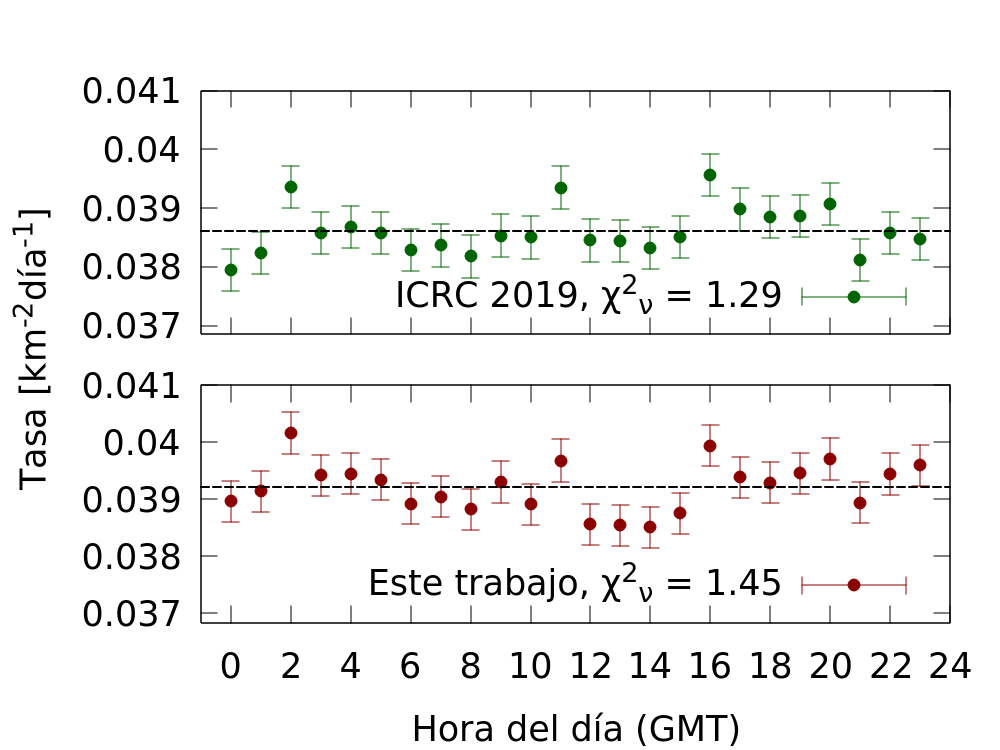
\includegraphics[width=\textwidth]{Graphs/2EeV_ICRC_2019_S38_S1000_expected.png}
                \caption{2005-2015} \label{fig:2EeV_expected}
                \end{subfigure}\\
                % \hspace{\fill}
                \begin{subfigure}[b]{0.5\textwidth}
                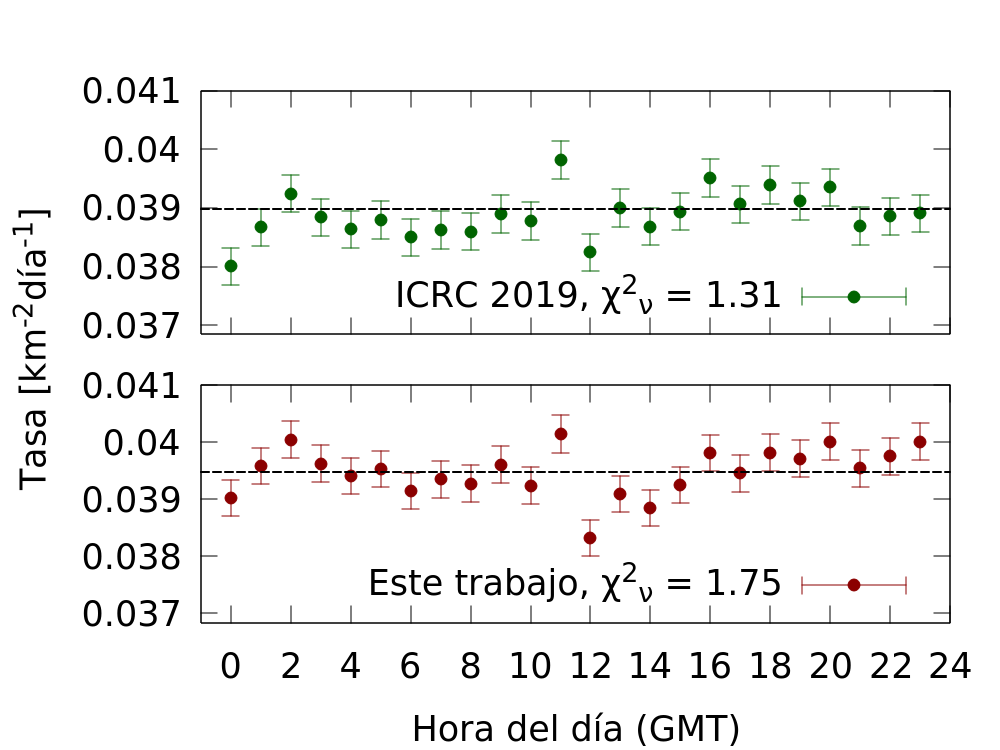
\includegraphics[width=\textwidth]{Graphs/2EeV_ICRC_2019_S38_S1000_expected_05_18.png}
                \caption{2005-2018}\label{fig:2EeV_expected_05_18}
                \end{subfigure}%
                \caption{Tasa de eventos por día para eventos de energía mayor a 2\,EeV para los datos de ICRC 2019 y la tasa de eventos obtenida con la reconstrucción de energía en este trabajo comparados en los periodos estudiados}\label{final}
        \end{figure}
Cabe aclarar que para la corrección de la energía para este trabajo, no se consideraron las posibles modulaciones de los valores del CIC o del posible cambio en los coeficientes de la Ec.\ref{eq:s38_energy}. Debido a que estos coeficientes son calibrados con eventos híbridos que son detectados durante la noche, donde las condiciones atmosféricas difieren de las condiciones promedios. Por ejemplo, en el caso de la densidad, durante la noche es aproximadamente $2\%$ mayor que el promedio.

% @@@@@@@@@@@@@@@@@@@@@@@@@@@@@@@@@@@@@@@@@@@@@@@@@@@@@@@@@@@@@@@@@@@@@@@@@@@@@
% @@@@@@@@@@@@@@@@@@@@@@@@@@@@@@@@@@@@@@@@@@@@@@@@@@@@@@@@@@@@@@@@@@@@@@@@@@@@@
% @@@@@@@@@@@@@@@@@@@@@@@@@@@@@@@@@@@@@@@@@@@@@@@@@@@@@@@@@@@@@@@@@@@@@@@@@@@@@
% @@@@@@@@@@@@@@@@@@@@@@@@@@@@@@@@@@@@@@@@@@@@@@@@@@@@@@@@@@@@@@@@@@@@@@@@@@@@@
% @@@@@@@@@@@@@@@@@@@@@@@@@@@@@@@@@@@@@@@@@@@@@@@@@@@@@@@@@@@@@@@@@@@@@@@@@@@@@
% @@@@@@@@@@@@@@@@@@@@@@@@@@@@@@@@@@@@@@@@@@@@@@@@@@@@@@@@@@@@@@@@@@@@@@@@@@@@@
% @@@@@@@@@@@@@@@@@@@@@@@@@@@@@@@@@@@@@@@@@@@@@@@@@@@@@@@@@@@@@@@@@@@@@@@@@@@@@
% @@@@@@@@@@@@@@@@@@@@@@@@@@@@@@@@@@@@@@@@@@@@@@@@@@@@@@@@@@@@@@@@@@@@@@@@@@@@@
% @@@@@@@@@@@@@@@@@@@@@@@@@@@@@@@@@@@@@@@@@@@@@@@@@@@@@@@@@@@@@@@@@@@@@@@@@@@@@
% @@@@@@@@@@@@@@@@@@@@@@@@@@@@@@@@@@@@@@@@@@@@@@@@@@@@@@@@@@@@@@@@@@@@@@@@@@@@@
% @@@@@@@@@@@@@@@@@@@@@@@@@@@@@@@@@@@@@@@@@@@@@@@@@@@@@@@@@@@@@@@@@@@@@@@@@@@@@
% @@@@@@@@@@@@@@@@@@@@@@@@@@@@@@@@@@@@@@@@@@@@@@@@@@@@@@@@@@@@@@@@@@@@@@@@@@@@@


% \section{Trabajos futuros}

% Vimos que las modulaciones del clima son parametrizadas mediante los coeficientes obtenidos en este y en otros trabajos de manera precisa. Durante la maestría se realizará un análisis de anisotropía con las energías corregidas por las condiciones atmosféricas mediante este trabajo y \cite{aab2017impact}. 
% Se analizará para distintos intervalos de energía por encima de 1 EeV, el primer armónico de ascensión recta en frecuencia solar y anti-sidérea, usando las  dos correcciones mencionadas. En estas dos frecuencias la señal debería ser menor a las fluctuaciones estadísticas, si las modulaciones espurias debidas a las condiciones atmosféricas están corregidas correctamente. En ese caso se puede realizar un análisis de Fourier estándar en la frecuencia sidérea para estudiar las anisotropías a grandes escalas angulares.

% %Se cuantificará las comparaciones entre las correcciones de \cite{aab2017impact} y de este trabajo, en intervalos por encima de 1\,EeV de energía, con el primer armónico en la ascensión recta en la frecuencia sidérea y anti-sidérea. Para este rango de energía también se estudiará la probabilidad de disparo de los tanques. 


% Por otra parte se analizarán las correcciones del clima en la estimación de la energía para los eventos reconstruidos  utilizando los disparos $ToTd$ y $Mop$,  que permiten detectar CRs de menor energía y dan lugar a un eficiencia máxima de disparo hasta  energías del orden de $1\,$EeV. Se comprobará si los parámetros del trabajo \cite{aab2017impact} son los adecuados  para estos eventos. Luego se estudiará la amplitud del primer armónico en la frecuencia solar y anti-sidérea para comprobar la ausencia de fluctuaciones espurias, antes de realizar análisis de anisotropía. 












%FAlta cuatificar ela comparacione entre los correcione ant y ahora es un estuidar en bins encima de un 1EeV de enrgía las anisotropias / EL primer armonico en la asencrecion recta en la freq sid y anti-sie

%Para ! está la probablilidad de trigger

%El paso sigu en primer lugar mirar los triggger nuevos ToTd mops ara ver si la corrcion si la correcion de l wea ant va bien para esos evenots y de nuevo constatar como funciona siendo el pr Ra en freq sid solar, para poder usar la anisotropia intrinsieca .

%Empezar a hacer analisis de anisotoropia con las dos correcciones
%Arriba de 2EeV. 
%abajo de full eff hay que ponerle una ocrecicion que dpende de la eff en fun de  E y ang
%tigger nueov con full detectas mas bajo pero menos estadistica
%hacer de  una corrcion con el mops con la effic. el tema es que la ef depende del error.
%